
%
% This is the LaTeX source for the instructions to authors using
% the LaTeX document class 'llncs.cls' for contributions to
% the Lecture Notes in Computer Sciences series.
% http://www.springer.com/lncs       Springer Heidelberg 2006/05/04
%
% It may be used as a template for your own input - copy it
% to a new file with a new name and use it as the basis
% for your article.
%
% NB: the document class 'llncs' has its own and detailed documentation, see
% ftp://ftp.springer.de/data/pubftp/pub/tex/latex/llncs/latex2e/llncsdoc.pdf
%
%%%%%%%%%%%%%%%%%%%%%%%%%%%%%%%%%%%%%%%%%%%%%%%%%%%%%%%%%%%%%%%%%%%


\documentclass[runningheads,a4paper]{llncs2e/llncs}

\usepackage{amssymb}
\setcounter{tocdepth}{3}
\usepackage{graphicx}
\usepackage{amsmath}

\usepackage{url}
\newcommand{\keywords}[1]{\par\addvspace\baselineskip
\noindent\keywordname\enspace\ignorespaces#1}

\usepackage{xspace}
%\newcommand{\ie}{\textit{i.e.,}\xspace}
%\newcommand{\eg}{\textit{e.g.,}\xspace}
%\newcommand{\vs}{\textit{v.s.}\xspace}

%

%\mainmatter  % start of an individual contribution

\usepackage{wrapfig}

\sloppy

%%% FORMAT DOCUMENT

\def\textfraction{0}
\def\floatpagefraction{1}
\def\topnumber{3}
\def\bottomnumber{3}
\def\totalnumber{3}
\def\topfraction{1}
\def\bottomfraction{1}

\usepackage[colorlinks]{hyperref}
%\usepackage[inner=2cm,outer=2cm,bottom=2cm,top=3cm]{geometry}
\usepackage{wrapfig}
\usepackage{subfigure}
\usepackage{xspace}
%%%%%%%%%%%%%%%%%%%%%%%%%%%%%%%%%%%%%%%%%
% Acronym of the proposal
\newcommand{\proposal}{DISCUTE\xspace}
%%%%%%%%%%%%%%%%%%%%%%%%%%%%%%%%%%%%%%%%%
%% TODO macros
\usepackage[textwidth=17mm]{todonotes}
  \newcommand{\customtodo}[4]{
        \todo[color=#2,inline,size=\small]{
                \ifx&#3&
                        \textbf{#1} #4
                \else
                        \textbf{#1$\Rightarrow$#3} #4
                \fi
        }
  }
\usepackage{ifthen}
\newboolean{WIP}
\gdef\ifwip{\ifthenelse{\boolean{WIP}}}
%\setboolean{WIP}{false}%
\setboolean{WIP}{true}%
\ifwip{
  \newcommand{\AL}[2][]{\customtodo{AL}{green!50}{#1}{#2}}
  \newcommand{\MS}[2][]{\customtodo{MS}{red!20}{#1}{#2}}
  \newcommand{\JP}[2][]{\customtodo{JP}{blue!20}{#1}{#2}}
  \newcommand{\FQ}[2][]{\customtodo{FQ}{brown!20}{#1}{#2}}
}{ % else if WIP = false
  \newcommand{\AL}[2][]{}
  \newcommand{\MS}[2][]{}
  \newcommand{\JP}[2][]{}
  \newcommand{\FQ}[2][]{}
}
%% End of todo macros
%%%%%%%%%%%%%%%%%%%%%%%%%%%%%%%%%%%%%%%%%
%% Italic abreviations, ...
\newcommand{\ie}[0]{\emph{i.e.},\xspace}
\newcommand{\vs}[0]{\emph{vs.}\xspace}
\newcommand{\eg}[0]{\emph{e.g.},\xspace}
\newcommand{\etal}[0]{\emph{et al.}\xspace}
\newcommand{\wrt}[0]{\emph{w.r.t.}\xspace}
\newcommand{\aka}[0]{\emph{a.k.a.}\xspace}
%%%%%%%%%%%%%%%%%%%%%%%%%%%%%%%%%%%%%%%%%



%%% Local Variables:
%%% mode: latex
%%% TeX-master: "main"
%%% End:


%\usepackage{titlesec}
%\titlespacing\subsubsection{0pt}{10pt plus 4pt minus 2pt}{0pt plus 2pt
% minus 2pt}[12pt]



\begin{document}
% first the title is needed
\title{VMPlaceS: A Generic Tool to Investigate and Compare VM Placement Algorithms}
\titlerunning{VMPlaceS - VM Placement Simulator}
% the name(s) of the author(s) follow(s) next
%
% NB: Chinese authors should write their first names(s) in front of
% their surnames. This ensures that the names appear correctly in
% the running heads and the author index.
%
\author{Adrien Lebre, Jonathan Pastor, Mario S\"udholt}
%
\authorrunning{A. Lebre, J. Pastor \and M. S\"udholt}
% (feature abused for this document to repeat the title also on left hand pages)

% the affiliations are given next; don't give your e-mail address unless you
% accept that it will be published
\institute{ASCOLA Research Group,
Mines Nantes / Inria / LINA, Nantes, France\\
\email{firstname.lastname@inria.fr}
 }

\maketitle

    Most current infrastructures for cloud computing leverage static
    and greedy policies for the placement of virtual machines. Such
    policies impede the optimal allocation of resources and the
    satisfaction of operational guarantees like service-level
    agreements. In recent years, more dynamic and often more efficient
    policies based, \eg on consolidation and load balancing
    techniques, have been developed and investigated. New policies are
    typically evaluated either using testbeds or \emph{in-vivo}
    experiments. However, due to the underlying complexity of cloud
    infrastructures, testbeds typically have to be tailored to
    specific restricted configurations and experiments on real
    infrastructures are necessarily of limited scale.

    In this article, we propose \vmps, a dedicated simulation
    framework to perform in-depth investigations of VM placement
    algorithms and compare them in a fair way. This framework, built
    on top of the \sg simulation platform, notably provides
    programming support to easy the implementation of placement
    algorithms and runtime support dedicated to load injection and
    execution trace analysis. \vmps supports the simulation of a large
    set of real-world configurations, while allowing researchers to
    conduct experiments at large scales. We also report on a
    validation of our framework by implementing and investigating
    representative algorithms for three classes of placement
    algorithms: centralized, hierarchical and fully-distributed ones.


%% Comment this line for submission
%\listoftodos

\section{Introduction}
\section{The VM Placement Problem}
\label{sec:vmpp}

A VMPP can be summarized in three-steps (see Figure
\ref{fig:scheduling_steps}): monitoring the resources usages,
computing a new schedule each time is it needed and applying the
resulting reconfiguration plan (\ie performing VM migration and
suspend/resume operations to realize to the new placement solution).
% that are mandatory to solve resource violations while optimizing resource usages).

\begin{figure}[ht]
\vspace*{-.2cm}
\begin{center}
        \subcapcentertrue
        \subfigure[Scheduling steps]{
        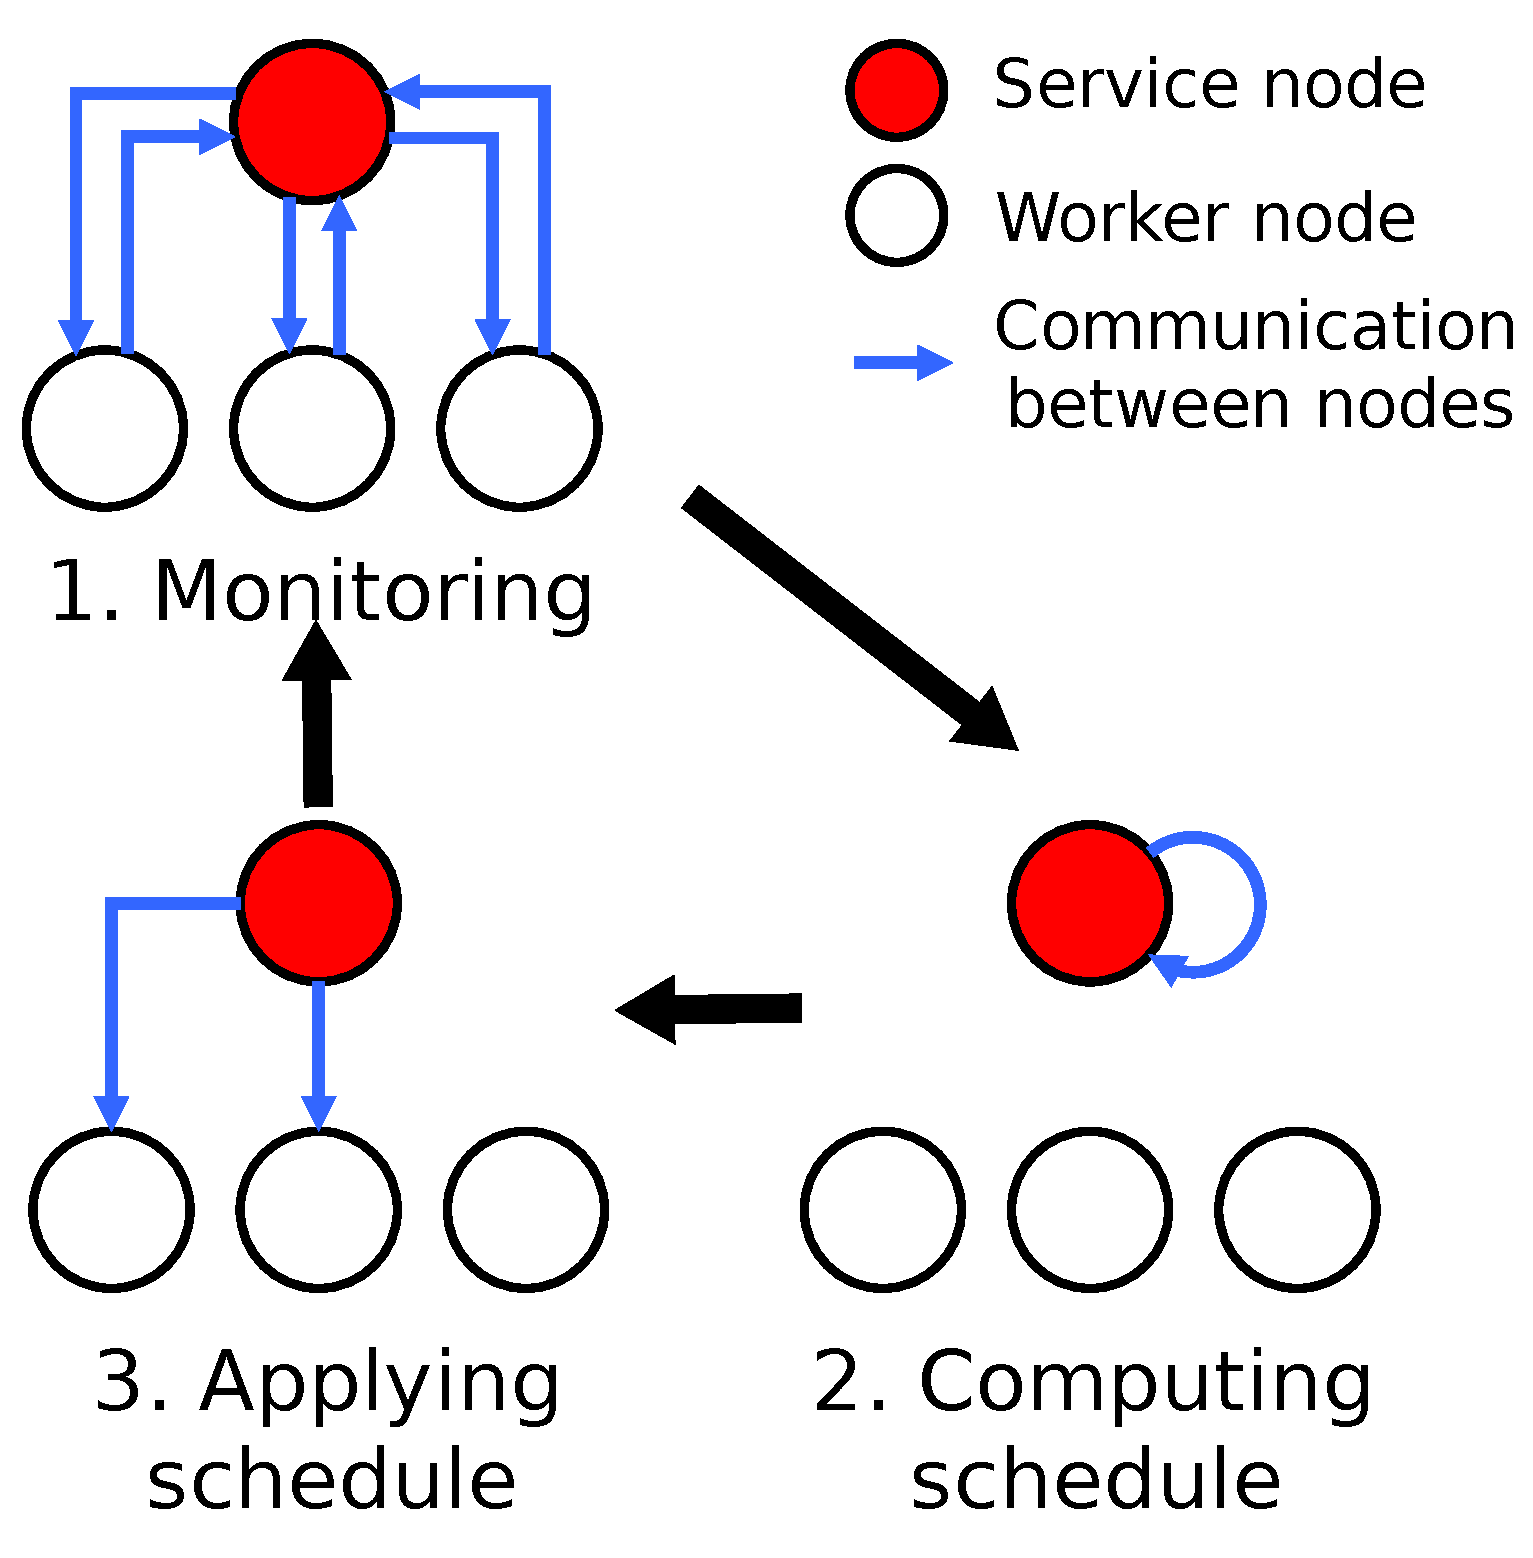
\includegraphics[width=.45\linewidth]{figures/scheduling_steps.pdf}
        \label{fig:scheduling_steps}}
        \subfigure[Workload fluctuations during scheduling]{
        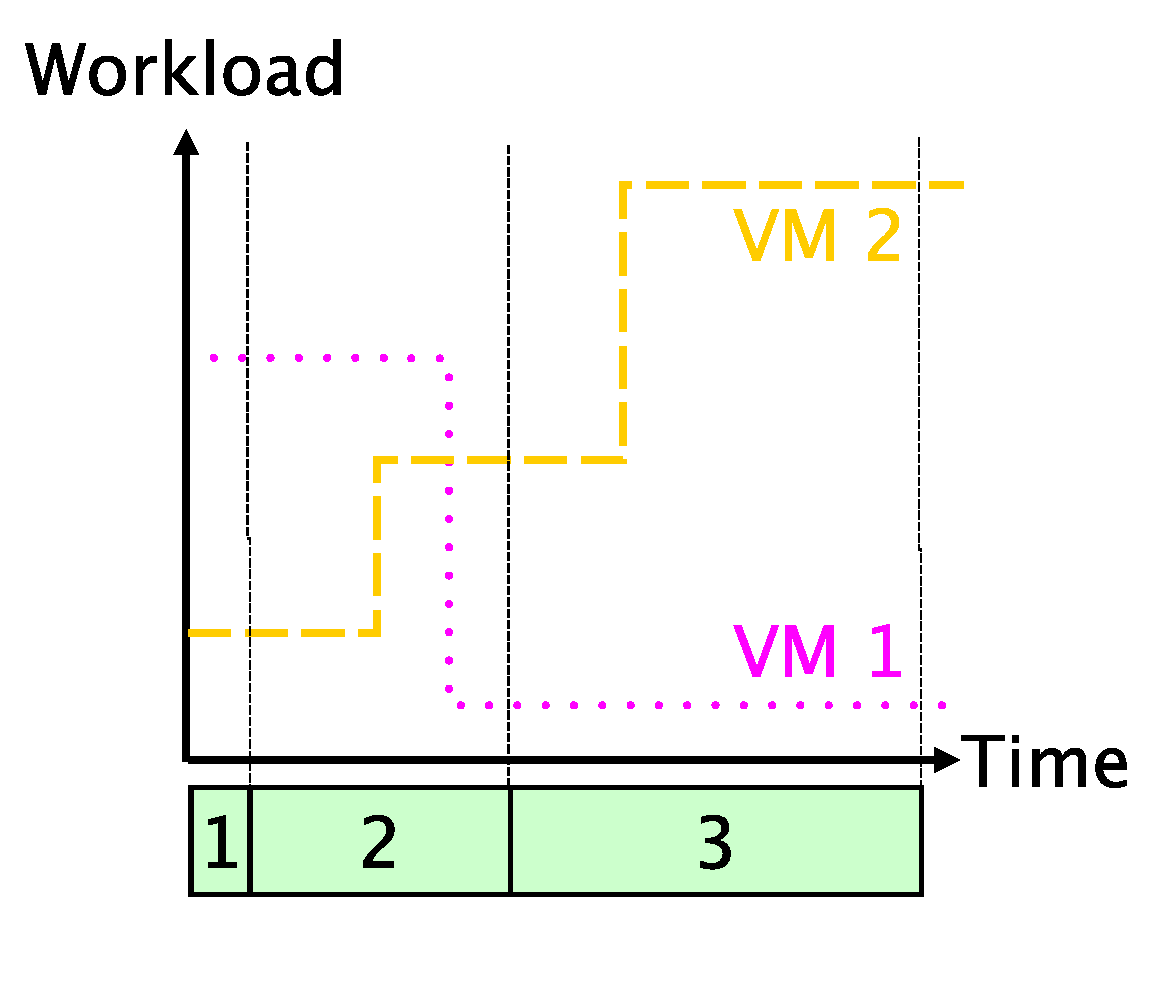
\includegraphics[width=.45\linewidth]{figures/workload_fluctuations2.pdf}
        \label{fig:workload_fluctuations}}
\vspace*{-.2cm}
\caption{VM scheduling Phases}
\end{center}
\label{fig:scheduling}
\vspace*{-.2cm}
\end{figure}
%

VMPP solutions stand and fall with their scalability, reliability and
reactivity of properties, because they have to maintain a placement
that satisfies the requirements of all VMs while optimizing the usage
of CC resources. For instance, a naive implementation of a
master/worker approach as described in
Figure~\ref{fig:scheduling_steps} would prevent workload fluctuations
to be taken into account during the computation and the application of
a schedule, potentially leading to artificial violations (\ie resource
violations that are caused by the VMPP mechanism). In other words, the
longer each phase,
% the longer the reconfiguration process,
the higher the risk that the schedule may be outdated when it is
computed or eventually applied, cf.\ the different loads during the
three phases in Figure \ref{fig:workload_fluctuations}. Similarly,
servers and network crashes can impede the detection and resolution of
resource violations if the master node crashes or if a group of VMs is
temporarily isolated from the master node.

VMPP solutions can only be reasonably evaluated if their behavior in
the presence of such adverse events can be analyzed. Providing a
framework that facilitates such studies and increases their
reproducibility is the main objective of \vmps.



\vspace*{-.05cm}
\section{Simgrid, a Generic Toolkit To Build Simulators}
\label{sec:sg}
%\vspace*{-.05cm}
%\AL[AL]{0.5page}

Developed for more than a decade,
% and used in a large number of studies described in mor than
% 100~publications,
\sg is a toolkit for the simulation of potentially complex algorithms
executed on large-scale distributed
systems~\cite{casanova:hal-01017319}.

To perform simulations, users should develop a \emph{program} and
define a \emph{platform} file and a \emph{deployment} file. The
\emph{program} leverages, in most cases, the \sg MSG API that allows
end-users to create and execute \sg abstractions such as processes,
tasks, VMs and network communications. The \emph{platform} file
provides the physical description of each resource composing the
environment and on which aforementioned computations and network
interactions will be performed in the \sg world.
% (host, CPU capacity, network topology and link capacities, etc.)
The \emph{deployment} file is used to launch the different \sg
processes defined in the \emph{program} on the simulated nodes.
% (at least the mapping between one process and one host is mandatory
% to start the simulation)
Finally, the execution of the program is orchestrated by the \sg
engine that internally relies on an constraint solver to correctly
assign the amount of CPU/network resources to each \sg abstraction
during the entire simulation.% (for a complete overview see ~\cite{casanova:hal-01017319}).


We chose to base \vmps on \sg
since (i) the latter's relevance in terms of performance and validity
has already been demonstrated~\cite{simgridpub} and (ii) because it
has been recently extended to integrate VM abstractions and a live
migration model \cite{Hirofuchi:2013:ALM:2568486.2568524}. In addition
to enabling researchers to control VMs in the same manner as in the
real world (\eg create/destroy VMs; start/shutdown, suspend/resume and
migrate them), the model implementing the precopy migration algorithm
of Qemu/KVM is the only one that successfully simulates the live
migration behavior by taking into account the competition arising in
the presence of resource sharing as well as the memory refreshing rate
of the VM, thus determining correctly the live migration time as well
as the resulting network traffic. These two capabilities were
mandatory to build \vmps.%our VM placement simulator toolkit.

\vspace*{-.2cm}
\section{VM Placement Simulator}
\label{sec:injector}
\vspace*{-.1cm}

%\AL[AL]{1.5 page}
The aim of \vmps is twofold:~(i) to relieve researchers of the burden of
dealing with VM creations and workload fluctuations when they evaluate
new VM placement algorithms and (ii) to offer the possibility to
compare them.
%
% The purpose of \vmps is to deliver a generic tool to evaluate new VM
% placement algorithms and offer the possibility to compare
% them. Concretely, it supports the management of VM creations and
% workload fluctuations.
% % as well as node apparitions/removals.
%  Researchers can
% thus focus on the implementation of new placement algorithms and
% evaluate how they behave in the presence of changes that occur during
% the simulation.
In the following we give an overview of \vmps and describe its
general functioning.

\vspace*{-.1cm}
%\subsection{Overview}
\paragraph{Overview}
\label{sec:overview}

\vmps has been implemented in Java by leveraging the \sg MSG API.
Although Java has an impact on the efficiency
of \sg, we believe its use is acceptable because Java offers important
benefits to researchers for the implementation of advanced scheduling
strategies, notably concerning the ease of implementation of new
strategies. As examples, we reimplemented the Snooze proposal in Java
and the DVMS proposal using Scala/Java.

\begin{wrapfigure}{r}{.48\linewidth}
\centering
\vspace*{-.6cm}
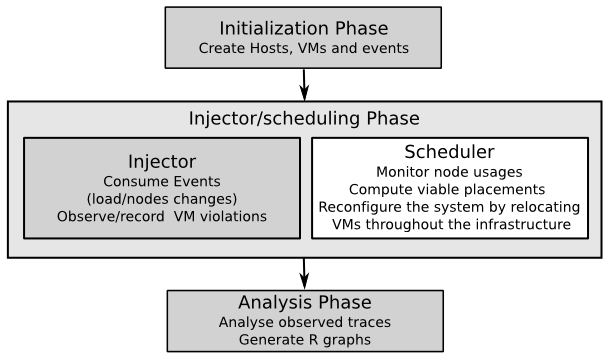
\includegraphics[width=.99\linewidth]{figures/VMPlaceS-workflow.pdf}
\vspace*{-.5cm}
\caption{\vmps's Workflow}
{\fontsize{7}{6}\selectfont  Gray parts correspond to the generic code while the white one
  must be provided by end-users. %The current version is released with
%  three different schedulers (centralized/hierarchical and
%  distributed).
}
\vspace*{-.8cm}
\label{fig:workflow}
\end{wrapfigure}
%
From a high-level view, \vmps performs a simulation in three phases:
(i) initialization (ii) injection and (iii) trace analysis (see Figure
\ref{fig:workflow}).  The initialization phase corresponds to the
creation of the environment, the VMs and the generation of the queue
of events (for the moment, VM load changes).
%
The
simulation is performed by at least two \sg processes, one executing
the \emph{injector}, which constitutes the generic part of the
framework and which, is in charge of injecting the events during the
execution of the simulation, and a second one executing the to-be-simulated
\emph{scheduling algorithm}.
%During the simulation the scheduling
%strategy is evaluated by injecting scheduling-relevant events.
%\AL[MS]{This sentence above is not accurate enough I? previously it
 % was : The
%\emph{injector} constitutes the generic part of the framework. It
%njects scheduling-relevant events during the execution of
%simulations. We should reformulate}
%Currently, the supported events are VM CPU load changes.
% node apparitions/removals that we use to simulate node crashes.
%
The last phase consists in the analysis of the collected traces in
order to gather the results of the simulation, notably by means of the
generation of figures representing, \eg resource usage statistics.

Researchers develop their scheduling algorithm by leveraging the \sg
MSG API and a more abstract interface that is provided by \vmps
and consists of the classes \texttt{XHost}, \texttt{XVM} and
\texttt{SimulatorManager}. The two former classes respectively
extend \sg's \texttt{Host} and \texttt{VM} abstractions while the
latter controls the interactions between the different components of
the VM placement simulator.  Throughout these three classes, users can
inspect, at any time, the current state of the infrastructure (\ie the
load of a host/VM, the number of VMs hosted on the whole
infrastructure or on a particular host, check whether a host is
overloaded, etc.).
%We have used \vmps in order to analyze three
%scheduling mechanisms, cf.\ Sec.~\ref{sec:vm-schedulers}, that
%represent three different software architecture models: centralized,
%hierarchical and fully-distributed models for VM placement.
%% TODO
%\MS{The
%  following point is too low-level and should not come here} Although
%we do not discuss that point due to space constraints, we emphasize
%that these three mechanisms enable us to deliver concrete examples of
%how the deployment file of \sg is automatically generated by leveraging
%a generic python script.  \AL{We should highlight that point in the
%  README.org}


%\begin{itemize}
%\item Entropy \cite{Hermenier:2009:ECM:1508293.1508300}, a centralized approach using a constraint programming approach to solve the placement/reconfiguration VM problem;
% \item Snooze \cite{feller:ccgrid12}, a hierarchical approach where
%   each manager of a group invokes Entropy to solve the
%  placement/reconfiguration VM problem. It is noteworthy that in
%   \cite{feller:ccgrid12}, Snooze is using a specific heuristic to solve the placement/reconfiguration VM problem. As the sake of simplicity, we have simply reused the entropy scheduling code.
%\item  DVMS \cite{quesnel:cpe2012}, a distributed approach that dynamically partitions the system and invokes Entropy on each partition.
% \end{itemize}

%\subsection{Initialization Phase}
%\\vspace*{-.15cm}
\paragraph{Initialization Phase}
In the beginning, \vmps creates $n$ VMs and assigns them in a
round-robin manner to the first $p$ hosts defined in the platform
file.  The default platform file corresponds to a cluster of $h+s$
hosts, where $h$ corresponds to the number of hosting nodes and $s$ to
the number of services nodes. The values $n$, $h$ and $s$ constitute
input parameters of the simulations (specified in a Java property
file).
%% TODO
% \AL[AL]{Update the size of the cluster autonomically by
%  leveraging p + s}
These hosts are organized in form of topologies, a cluster topology
being the most common one. It is possible, however, to define more
complex platforms to simulate, for instance, federated data center scenarios.
%Note that $s$ can be equals to 0 if the
%scheduling strategy is directly executed on the hosting nodes.

Each VM is created based on one of the predefined VM classes. A VM
class corresponds to a template specifying the VM attributes and its
memory footprint. Concretely, it is
% described as
% \texttt{nb\_cpu:ramsize:net\_bw:mig\_speed:mem\_speed}
defined in terms of five parameters: the number of cores
\texttt{nb\_cpus}, the size of the memory \texttt{ramsize}, the
network bandwidth \texttt{net\_bw}, the maximum bandwidth available
migrate it \texttt{mig\_speed} and the maximum memory update speed
\texttt{mem\_speed} when the VM is consuming 100\% of its CPU
resources.
Available classes
are defined in a specific text file that can be modified according to
the user's needs.
As pointed out in Section \ref{sec:sg}, the memory update
speed is a critical parameter that governs the migration time as well
as the amount of transferred data.
By giving the possibility to define
VM classes, \vmps allows researchers to simulate different kinds of
workload (\ie memory-intensive vs non-intensive workloads), and thus
analyze more realistic CC problems.

%\MS{Follows a low-level mechanism!}
% TODO not addressed yet. This text should appear in the README
%At creation time
%of a VM, a process selects one class (\ie one line) in the file
%randomly. Hence, if a user wants to favor a specific class, he can
%simply repeat the line of the class several times.
%
Finally, all VMs start with a CPU consumption of 0 that will evolve
during the simulation in terms of the injected load as explained
below.

Once the creation and the assignment of VMs completed, \vmps spawns at
least two SG processes, the \emph{injector} and the launcher of the
selected scheduler.  The first action of the \emph{injector} consists
in creating the different event queues and merge them into a global
one that will be consumed during the second phase of the simulation.
In the current release, \vmps generates one queue of \emph{CPU load change} events.
%and
%\emph{node crash} events.
%\todo{Before apparitions/ removals}
% The former consists in changing the load of a VM by creating and
% assigning a new \sg task in the VM while the second aims at
% simulating crashes.
%
% Changing the load of a VM has a direct impact of its memory update
% speed and thus on the time to migrate it between two hosts.
The \emph{CPU load change} event queue is generated in order to change the
load of each VM every $t$ seconds on average. $t$ is a random variable
that follows an exponential distribution with rate parameter
$\lambda_t$ while the CPU load of a VM evolves according to a Gaussian
distribution defined by a particular mean ($\mu$) as well as a
particular standard deviation ($\sigma$). $t$, $\mu$ and $\sigma$ are
provided as input parameters of a simulation.  As the CPU load can
fluctuate between 0 and 100\%, \vmps prevents the assignment of
nonsensical values when the Gaussian distribution returns a number
smaller than 0 or greater than 100. Although this has no impact on the
execution of the simulation, we emphasize that this can
reduce/increase the effective mean of the VM load, especially when
$\sigma$ is high.  Hence, it is important for users to specify
appropriate values.
%% TODO
%\AL[AL]{A binomial law would have solved this issue: too late too bad :(}
%Although this can have an impact on the
%effective mean, especially when $\sigma$ is high, we believe it was
%non appropriated to request it is easier for end-users to specify $\mu$ and
%$\sigma$ parameters than
Furthermore, each random process used in \vmps is initialized with a
seed that is defined in a configuration file. This way, we can ensure
that different simulations are reproducible and may be used to
establish fair comparisons.

%The \emph{node crash} event queue is generated in order to turn off a
%node every $f$ seconds on average for a duration of $d$ seconds.
%Similarly to the $t$ value above, $f$ follows an exponential
%distribution with rate $\lambda_f$. $f$ and $d$ are also provided as
%input parameters of a simulation.

Finally, we highlight that adding new events can be
done by simply defining new event Java
classes implementing the \texttt{InjectorEvent} interface and by
adding the code in charge of generating the associated queue. Such a
new queue will be merged into the global one and its events will then be
consumed similarly to the \emph{CPU Load} ones.% during the \emph{injector phase}.
As an example, the next release of \vmps will integrate   \emph{node
  apparition/removal events} that will be used to simulate crashes.

%\vspace*{-.1cm}
%\subsection{Injector Phase}
\paragraph{Injector Phase}
Once the VMs and the global event queue are ready, the evaluation of
the scheduling mechanism can start. First, the injector process
iteratively consumes the different events that represent, for now, load changes of a VM.
Changing the load of
a VM corresponds to the creation and the assignment of a new \sg task
in the VM. This new task has a direct impact on the time that will be
needed to migrate the VM as it increases or decreases the current CPU
load and thus % the percentage of
its memory update speed.
% \MS[AL]{Is the above paragraph clear enough?}
% that is indicated by the \texttt{mem\_speed}
%% parameter given in the class description.
%When a node is turning off, the VMs that were running on that node are
%temporarily discarded, \ie they are hidden and cannot be accessed
%until the node comes back to life. This way, the scheduler cannot
%handle them.
 %\AL[AL, MS, JP]{This is ugly but unfortunately the true,
 % it will be better to reassign those VMs on other nodes, but which
 % one?  }
%We leave for future work other approaches that can better
%match realistic scenarios such as turning off the VMs and
%reprovisioning them on other nodes.
%

Based on the scheduler decisions, VMs will be suspended/resumed
or relocated on the available hosts to meet scheduling objectives. % and SLA guarantees.
Note that users must implement the algorithm in
charge of solving the VMPP but also the code in charge of applying
reconfiguration plans by invoking the appropriate methods available
from the \texttt{SimulatorManager} class. This step is essential as
the reconfiguration cost is a key element of dynamic placement
systems.

% \MS[AL]{maybe it is better to prevent the access to Xhost
%   and XVM methods that can change the Simulator States. Hence, we
%   should enforce the access only through the SimulatorManager class?
%   What do you think? Yes, would be cleaner. Can we just present the
%   interface as such? Or not talk about the direct possibility?}
Last but not least, it is noteworthy that \vmps really invokes the
execution of each scheduling solver to get the effective
reconfiguration plan.  That is, the computation time that is observed
is not simulated but corresponds to the effective one, only the
workload inside the VMs and the reconfiguration operations (\ie
suspend/resume and migrate)  are simulated in
\sg. It is hence mandatory to propagate the effective computation time into
the \sg engine.%
% The following is IMO a technical detail
% by invoking a \texttt{wait} call of the MSG interface.

\vspace*{-.2cm}
%\subsection{Trace Analysis}
\paragraph{Trace Analysis}
\label{subsec:traces-analysis}

The last step of \vmps consists in analyzing the information that has
been collected during the simulation.
% in order to understand and compare the behavior of the different
% algorithms.
This analysis is done in two steps. First, \vmps records several
metrics related to the platform utilization % throughout the simulation
by leveraging an extended version of \sg's TRACE
module\footnote{\url{http://simgrid.gforge.inria.fr/simgrid/3.12/doc/tracing.html}}.
This way, visualization tools that have been developed by the \sg
community, such as PajeNG~\cite{pageng:www}, may be used. Furthermore,
our extension enables the creation of a JSON trace file, which is used to generate several figures, using the R
statistical environment~\cite{R:Bloomfield:2014},
about the resource usage during the simulation.

By default, \vmps records the load of the different VMs and hosts, the
appearance and the duration of each violation of VM requirements in
the system, the number of migrations, the number of times the
scheduler mechanism has been invoked and the number of times it
succeeds or fails to resolve non-viable configurations.
%
Although these pieces of information are key elements to understand
and compare the behavior of the different algorithms, we emphasize
that the TRACE API enables the creation of as many variables as
necessary, thus allowing researchers to instrument their own algorithm
with specific variables that record other pieces of information.

\section{Dynamic VMPP Algorithms}
\label{sec:vm-schedulers}
\vspace*{-.2cm}
To illustrate the interest of \vmps, we implemented three dynamic VM
placement mechanisms: a centralized one based on the Entropy
proposal~\cite{Hermenier:2009:ECM:1508293.1508300}, a hierarchical one
based on Snooze~\cite{feller:ccgrid12}, and a fully-distributed one
based on DVMS~\cite{quesnel:cpe2012}.
%\MS{We should differentiate more clearly between the complete VMPP
 % system and the solver.}
%
These systems enable, if it is possible,  the resolution  of violations in form of
overloaded nodes. A host is overloaded when the VMs try to consume
more than 100\% of the CPU capacity of the host. In such a case, a
resolution algorithm looks for a reconfiguration plan that can lead to
a viable configuration. For the sake of
simplicity, we chose to use the latest solver developed as part of the Entropy
framework~\cite{hermenier:cp11} in the three systems as this resolution algorithm.
The Entropy solver evaluates different viable configurations until  it
reaches a predefined timeout.
% Giving up consolidation optimality in favor of scalability, this
% algorithm provides a ``repair mode'' that enables the correction of VM
% requirement violations. The optimal solution is a new placement that
% satisfies the requirements of all VMs while minimizing the cost of the
% reconfiguration.
Once the timeout has been triggered, the algorithm returns the best
solution among the ones it finds and applies the associated
reconfiguration plan by invoking live migrations in the simulation
world.
%
% Although using the Entropy VMPP solver implies a modification from the
% original Snooze proposal, we highlight that our goal is to
%
% and thus we believe that such a modification is acceptable as it
% does not change the global behavior of Snooze

%Simulating these three VMPP systems illustrates the capabilities of
%\vmps. Moreover, by conducting such a comparison, we also investigate
%the pros and cons of the three architecture models on which these
%proposals rely on.% (\ie centralized, hierarchical and distributed).

In the remainder of this section, we present an overview of the
three systems, showing, in particular, that the extended abstractions
for hosts (\texttt{XHost}), VMs (\texttt{XVM}) and the functions of
the \sg MSG API enabled us to develop them in a direct and natural
manner.

%\subsection{Entropy-based Centralized Approach}
\subsubsection{Entropy-based Centralized Approach}
\label{subsec:entropy}
The centralized VM placement mechanism consists in one single \sg
process deployed on a service node. This process implements a simple loop that
iteratively checks the viability of the current configuration by
invoking the aforementioned VMPP solver with a predefined
frequency.
% $p$ is defined as an input parameter of the simulation.
% \AL{Should we explain the issue right now or not if we add VMPP section}
% Indeed, during
% the computation and the application of a schedule, the algorithm does
% not enforce QoS properties anymore, and thus cannot react quickly to
% violations. Second, since the manipulation of VMs is costly, the time
% needed to apply a new schedule is particularly important: The longer
% the reconfiguration process is, the higher is the risk that the schedule may
% be outdated, due to the workload fluctuations, when it is eventually
% applied.
% \vmps enables researchers to investigate such concerns in-depth.
%
% As the Entropy proposal does not provide a specific mechanism for the
% collection of resource usage information but simply uses an external
% tool (namely ganglia), we had two different ways to implement the
% monitoring to process: either by implementing additional asynchronous
% transmissions as a real implementation of the necessary state updates
% would proceed or, in a much more lightweight manner,
The resource usage is monitored through direct accesses
% by the aforementioned process
to the states of the hosts and their respective VMs.
%, while accounting for communication overheads explicitly.
%\AL[MS]{Not sure I understood  what you would say ?}
% induced by communication in the ``real'' implementation, for
% instance, can be easily added as part of the lightweight
% simulation. We have implemented this lightweight variant for the
% monitoring
%
% Regarding fault tolerance, similarly to the Entropy proposal, our
% implementation does not provide any failover mechanism.
%
% as mentioned in Section \ref{subsec:traces-analysis},
We also monitor, for each iteration, whether the VMPP solver succeeds
or fails. In case of success, \vmps records the number of migrations
that have been performed, the time it took to apply the
reconfiguration and whether the reconfiguration
led to new violations.

%\subsection{Snooze-based Hierarchical Approach}
\subsubsection{Snooze-based Hierarchical Approach}
\label{subsec:snooze}
\AL[MS]{1.5 pages}

We now present the Snooze framework for VM
management~\cite{feller:ccgrid12} as a second case study of how
to implement and simulate advanced algorithms.

\subsubsection{Overview}

We first briefly present the Snooze architecture summarizing its main
characteristics from its presentation~\cite{feller:ccgrid12} and
additional info stemming from personal communications of the Snooze
developers and its implementation~\cite{snoozedev14,snoozeweb}.
\begin{figure}
  {\centering ~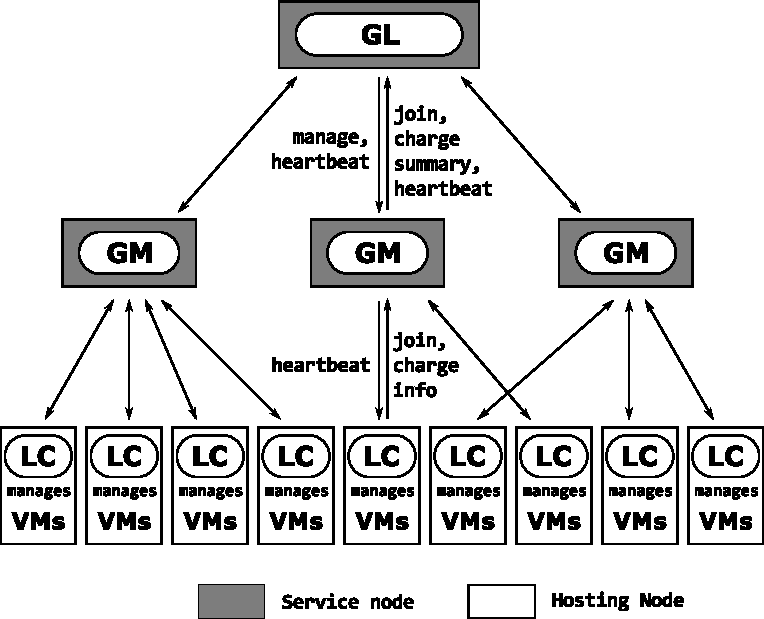
\includegraphics[width=.95\linewidth]{figures/snoozearch.pdf}}
  \caption{Overview of Snooze's architecture}
  \label{fig:snoozearch}
\end{figure}

\paragraph{Architecture}

Snooze harnesses a hierarchical architecture in order to support load
balancing and fault tolerance, see Fig.~\ref{fig:snoozearch}. At the
top of the hierarchy, a \emph{group leader (GL)} (that is installed on
a service node in our simulation) centralizes information about the
whole cluster by keeping summary information about all \emph{group
  managers (GMs)} (also installed on service nodes in our simulation)
that constitute the intermediate layer of the hierarchy. GMs manage a
number of \emph{local controllers (LCs)} (installed on an ordinary
node) and manages the VMs assigned to that node. During execution,
higher-level components periodically send heartbeats to lower-level
components; monitoring information, \eg on the system load, is also
sent periodically in the opposite direction. In order to propagate
information down the hierarchy, Snooze relies on hardware support for
multicast communication. Finally, a number of replicated entry points
allows clients to contact the GL, \eg in order to submit new VMs for
integration into the system.

\paragraph{Algorithms}
\label{sec:snoozeAlgs}

Apart from the handling of faults (described below), two types of
algorithms are of major importance for the administration of the
Snooze architecture: the algorithms that enable components to
dynamically enter the system and the algorithms that propagate info
between the components.

A GL is created, if it does not exist, by promotion of a GM that is
selected according to some leader election algorithm. When a GM joins
a cluster, it starts listening on a predefined channel for the
heartbeat of the GL and registers once it has received the
heartbeat. New LCs first also wait for the GL heartbeat, request a GM
assignment from the GL and register at the GM assigned to them.

Information that is passed within the system consists in periodic
heartbeat message from the GL, GMs and LCs as well as, also periodic,
charge information from LCs sent to their respective GMs and summary
charge info sent by GMs to the GL.


\paragraph{Fault tolerance}

GLs, GMs and LCs may fail during the system execution. System
components identify that a node on the corresponding higher-level node
has failed (the GL in case of a GM, a GM in the case of an LC) in an
asynchronous fashion through the lack of heartbeat messages.

In the case of a GL failure, one of the GMs becomes the new GL, stops
its GM activities and prevents the LCs it manages so that they can
start rejoining the system. If a GM fails, the GL and the LCs it has
managed will become aware of it based on the lack of heartbeats,
update its data structures and, for the LCs, rejoin the system. If an
LC fails, its GM will finally learn of it due to the missing heartbeat
and charge information of the LC. The GM will then remove the LC from
its data structures.

\subsubsection{Simulation using Simgrid}

Snooze can be simulated using our model and tool support in a direct
and natural manner. The extended abstractions \MS[MS]{Refer to
  Sec.~\ref{sec:overview}} for hosts (\texttt{XHOST}) and VMs
(\texttt{XVM}) provide low-level facilities for scheduling algorithms
that facilitate the implementation of the Snooze simulation. We have
harnessed these facilities in order to implement core characteristics
of Snooze: the monitoring of all VMs that are part of an LC and the
migration of all VMs of the set of LCs that are managed by a GM.

The remaining concepts and algorithms of Snooze are implemented using
means of our framework, the facilities provided by Simgrid and
standard Java mechanisms. Communication between Snooze actors is
implemented based on Simgrid's primitives for, mainly asynchronous,
event handling; in particular, hardware-supported multicast
communication that is used, for example, in order to relay heartbeats
is implemented as a dedicated actor that manages a state representing
GL and GM heartbeat groups and relaying heartbeat events.

The Snooze simulation uses, as its original counterpart, a
multi-threaded implementation in order to optimize reactivity even for
large groups of LCs (or GMs) that have to be managed by one GM (or
GL).

\subsubsection{Variants}
\label{sec:snoozeVariants}

Our simulation framework facilitates the simulation of variants of
placement algorithms. In the following, we present three non-trivial
variants that we have implemented and explored: a variant of the
assignment algorithm of LCs to GMs, periodic vs.\ reactive scheduling,
and a variant of the algorithms of how GMs and LCs join the system.


\paragraph{Assignment of LCs to GMs}

LCs are assigned to GMs by the GL as part of the LC join protocol. In
Snooze's native implementation LCs are assigned in a round-robin
fashion to the known GMs. If GMs join (and leave) the system at the
same time as LCs, a round-robin strategy at join time, however, does
not ensure an even distribution. This may happen, for instance at
startup time of the system, when new GMs and LCs enter the system, or
in case of failures, which trigger GM and LC joins. In order to
evaluate the imbalance resulting from a round-robin strategy (as well
as others) we have implemented the LC assignment protocol in a modular
fashion and applied it in diverse highly-dynamic settings in which GMs
and LCs enter the system at the same time. Furthermore, we have
implemented a best-fit strategy that assigns LCs to GMs with minimal
load or to GMs with the smallest number of assigned LCs (if several
GMs with minimal load exist). The best-fit strategy can significantly
improve the scheduling characteristics of hierarchical placement
algorithms as shown by the experimental data presented in
Sec.~\ref{sec:snoozeVariantsEval}. Furthermore, it should always be
at least as good as the round-robin strategy (the corresponding proof
is left to future work).


\paragraph{Periodic vs.\ reactive scheduling}

Snooze~\cite{feller:ccgrid12} schedules VMs in a periodic fashion:
after a fixed time period a GM calls the scheduler in order to resolve
resource conflicts among the LCs it manages. The information whether a
resource conflict has to be handled is taken based on the summary
information that is periodically sent by the LCs to the GM.

We have provided an alternative, reactive, strategy to scheduling: as
soon as they occur, LCs avert their GMs of resource conflicts; the GMs
then initiate scheduling. Implementing this reactive scheme can be
done using our framework in two manners: either by implementing
additional asynchronous transmissions as a real implementation of the
necessary state updates would proceed or, in a much more lightweight
manner, through direct accesses by the GMs to the states of their
respective LCs. While the latter does not mimic a real implementation
closely, it can be harnessed to yield a valid simulation: delays
induced by communication in the ``real'' implementation, for instance,
can be easily added as part of the lightweight simulation. We have
implemented this lightweight variant of reactive scheduling.


\paragraph{Variants of the join algorithms}

The join algorithms, see Sec.~\ref{sec:snoozeAlgs}, are crucial to the
correctness of Snooze for two main reasons: (i) they have to be
efficient because they can easily form a bottleneck if large numbers
of LCs (GMs) have to be registered at a GM (LC); (ii) they are
multi-phase protocols whose correctness especially in the presence of
faults is difficult to ensure.

In order to investigate the corresponding trade-offs, we have used our
framework to implement join algorithms that may be interrupted at any
time, repeat the the on-going phase a number of times before
reinitiating, if necessary, the entire protocol. Furthermore, the join
protocol is parameterized, \eg, in the number of threads used to
handle registration requests.

Finally, our framework has enabled us to test another aspect of
Snooze's join algorithm as presented by
Feller~\etal.~\cite{feller:ccgrid12},
\MS[MS]{If we succeed to perform the experiment comparing both
  approach, this paragraph should be highlighted.}
a strategy we call the GM rejoin
strategy (GRJ): all GMs should rejoin if a new GM enters the
system. While GRJ supports a form of load balancing (because all LCs
are reassigned to the new set of GMs), our simulation has shown that
this strategy significantly increases the time necessary for
registering GMs and LCs compared to a simpler strategy that does not
modify existing GMs in case a new GM enters the system. This handicap
is particularly pronounced if joins of GMs may be interrupted due to
faults. Concretely, experiments involving 20 GMs and 200 LCs have
shown that this strategy often multiplies the time necessary to join
all 220 components by 10 or more compared to the simple join
strategy. While the qualitative result that the more complex strategy
presented in the paper results in a more time-consuming join process
is not very surprising, the extent of the resulting degradation was
surprising.



%%% Local Variables:
%%% mode: latex
%%% TeX-master: "main"
%%% End:


%\subsection{DVMS-based Distributed Approach}
\subsubsection{DVMS-based Distributed Approach}
\label{subsec:dvms}
% As the third use-case, we have implemented the
DVMS (Distributed Virtual Machine Scheduler)~\cite{quesnel:cpe2012} enables the
cooperative and fully-distributed placement of
VMs. A DVMS agent is deployed on each node in order to manage the VMs on
the node and collaborate with (the agents of) neighboring nodes.
Agents are defined on top of an overlay communication network that
defines the node-neighbor relation.
% and can be structured (using, \eg
% Chord~\cite{stoica:2001:sigcomm01}) or unstructured.  For this
% study,
We have implemented a simple % but effective
unstructured overlay that enables the agents to collaborate
% without side effects: when necessary, \eg in case of node failures,
% the overlay
by providing a link to a neighbor %of a node
on the latter's request.
% \MS[AL, JP]{A bit short. What about an architecture figure (as for
%  Snooze?)}




% \paragraph{Iterative Scheduling Procedure.}
% \label{sec:ISP}
% \AL[MS,JP]{if we succeed to have only one or two subsections in
%   Snooze, we should do the same here.}

Fig. \ref{fig:dvms_pte} depictes the DVMS algorithm.
When a node N\(_{\textit{i}}\) detects that it cannot provide enough
resources for its hosted VMs, %(\ie VMs hosted on the server require more
%resources than available),
an \emph{Iterative Scheduling Procedure
  (ISP}) is started:
%
%When a node N\(_{\textit{i}}\)
%detects that it cannot provide enough resources for its hosted VMs,
it initiates a partition, reserving itself to solve the problem (sse
Fig.~\ref{fig:dvms_pte_1}).
Then, its
closest neighbor % , as defined by the network overlay,
is considered.
%
%
%
If this neighbor, N\(_{\textit{i+1}}\),
is already part of another partition, the next neighbor is considered.
%\AL[MS]{Not clear enough, its next neighbor ?}
Otherwise, N\(_{\textit{i+1}}\)
joins the partition (see Fig.~\ref{fig:dvms_pte_2}) and becomes the
partition leader.
% % If the partition is not valid anymore (\eg because the workload of the
% % partition's VM has decreased), N\(_{\textit{i+1}}\)
% % cancels the reservations, destroys the partition and thus frees its
% % nodes for another problem solving procedure.
% % %
% % On the contrary, if the procedure is still valid, N\(_{\textit{i+1}}\)
% % notifies members of the partition that it has become the new
% % leader.
%
The other nodes involved in the partition then send it information about their
capacities and current load. The leader, in turn, starts a scheduling
computation looking for a reconfiguration within the current
partition. If no solution is found, the same algorithm is applied to
the next node N\(_{\textit{i+2}}\).
%
% % In the extreme case a partition may grow until all resources in a
% % cluster contribute to the resolution of its resource scheduling
% % problem.
This approach constructs small parititions in a highly parallel
manner (Fig.~\ref{fig:dvms_pte_3}), thus significantly accelerating
the scheduling process and thus the reactivity criteria.

Most of the DVMS code has been coded in SCALA leveraging the Java
primitives of \sg for the communications between the different DVMS agents.

\begin{figure}[t]
\vspace*{-.6cm}
\subfigure[]{
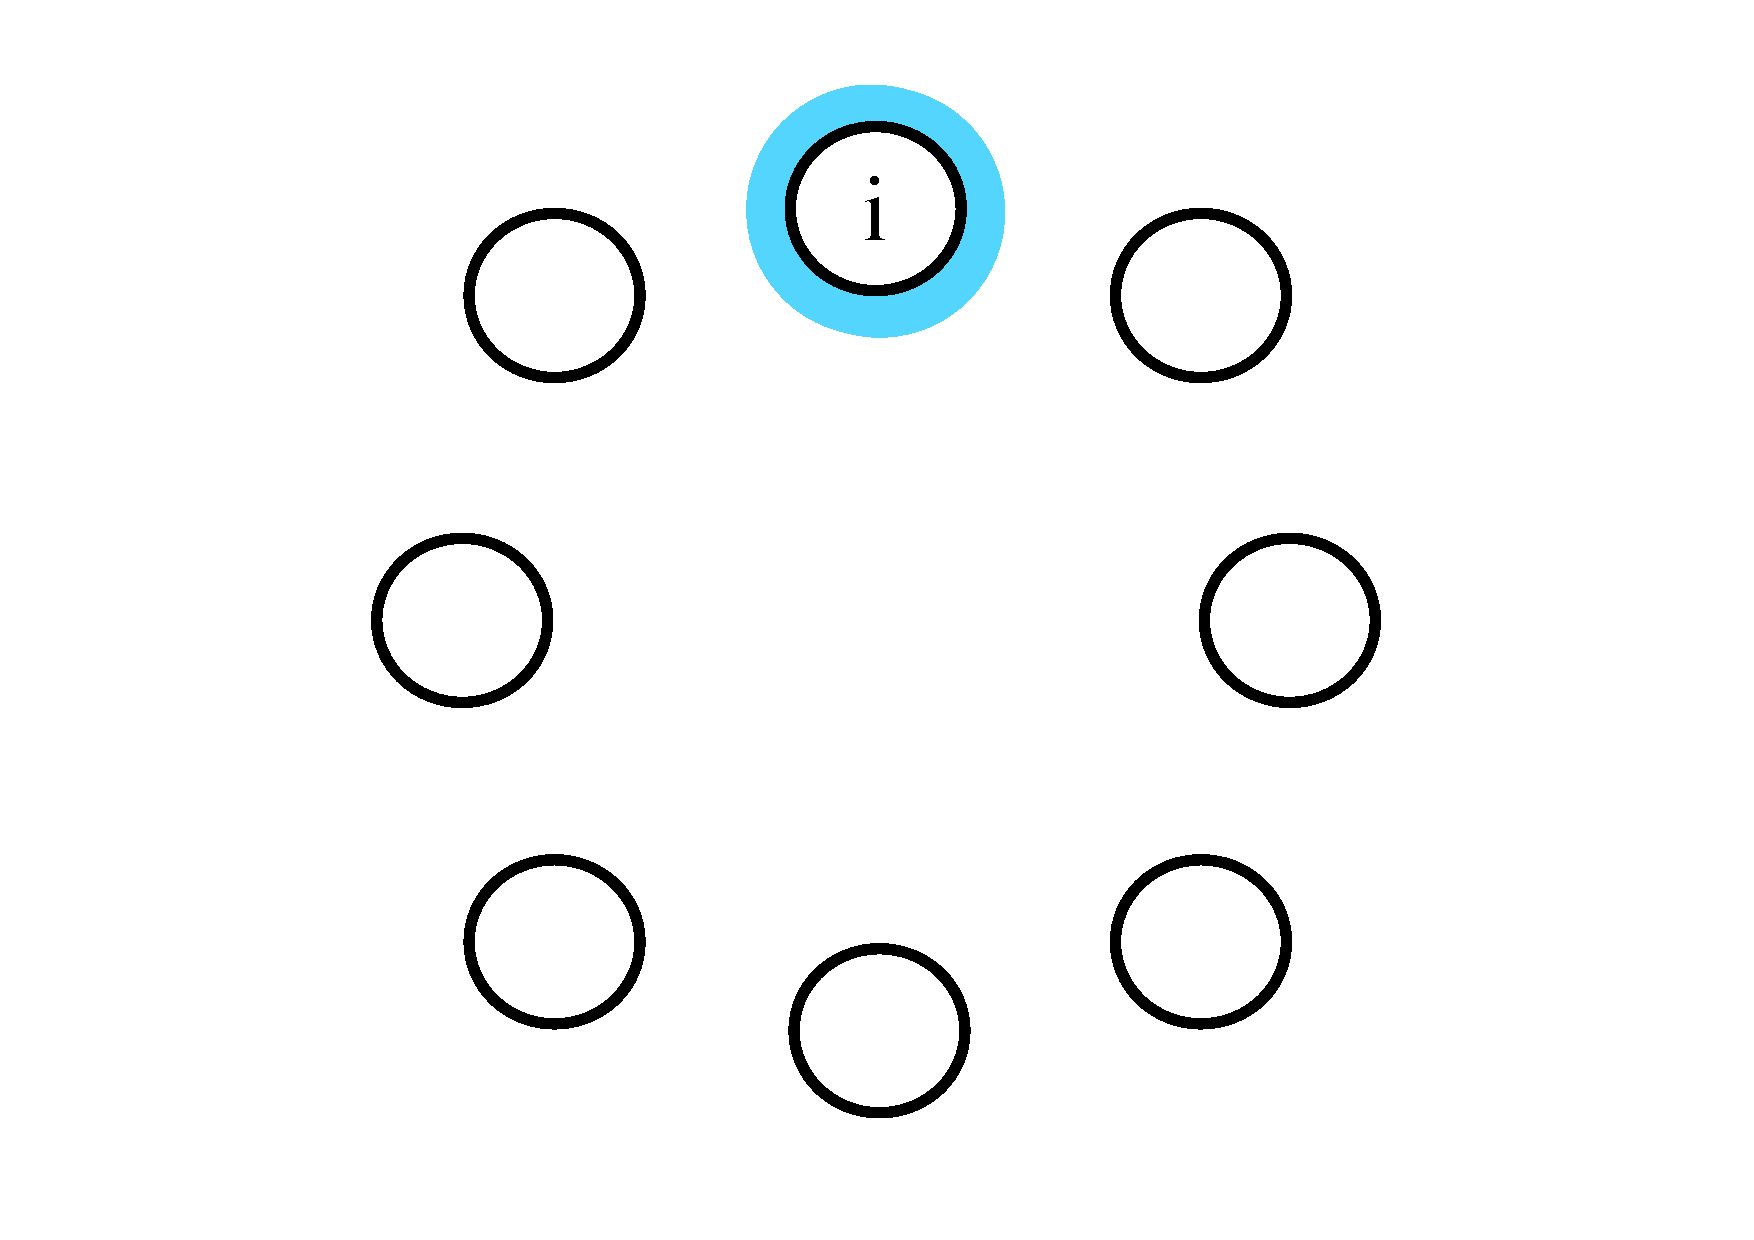
\includegraphics[width=2.7cm]{./figures/fig-24.pdf}
\label{fig:dvms_pte_1}}
%
\subfigure[]{
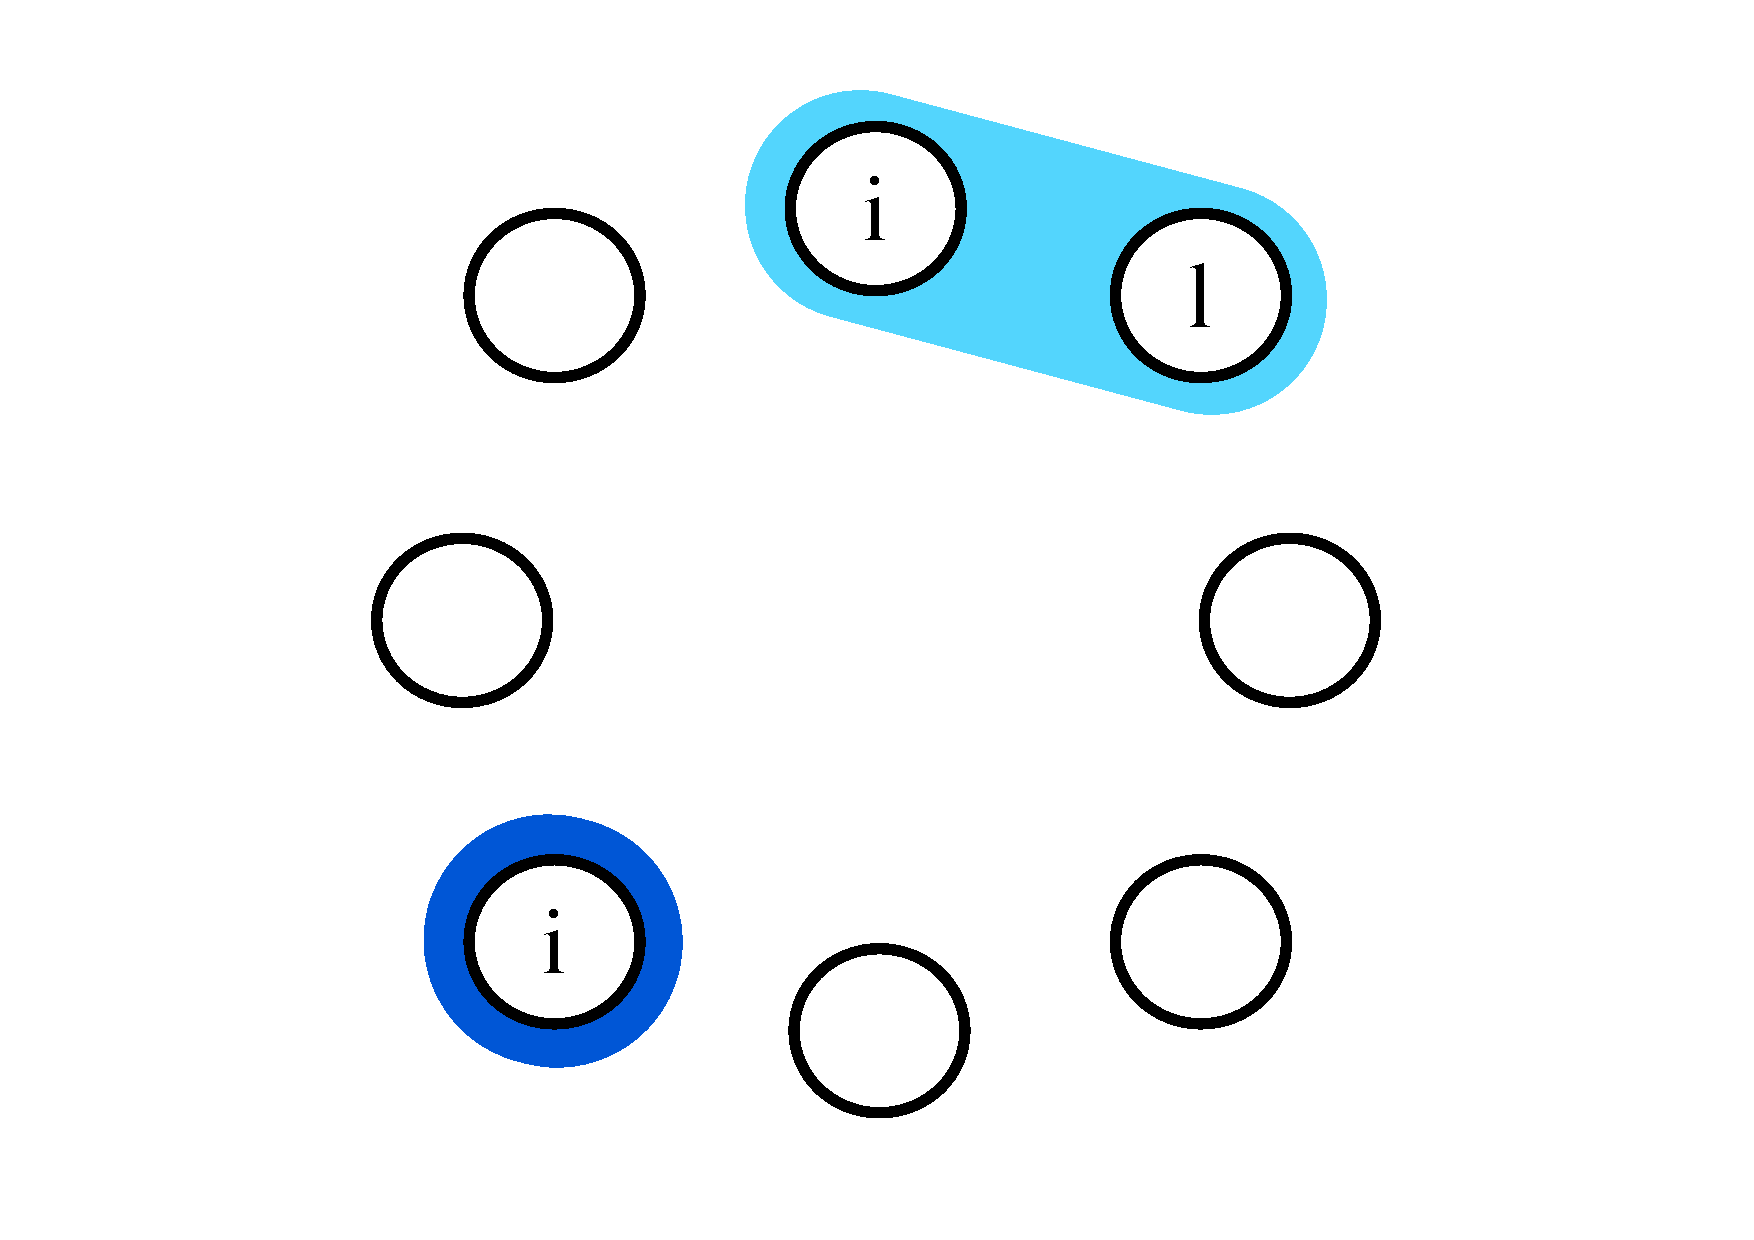
\includegraphics[width=2.7cm]{./figures/fig-25.pdf}
\label{fig:dvms_pte_2}}
%
\subfigure[]{
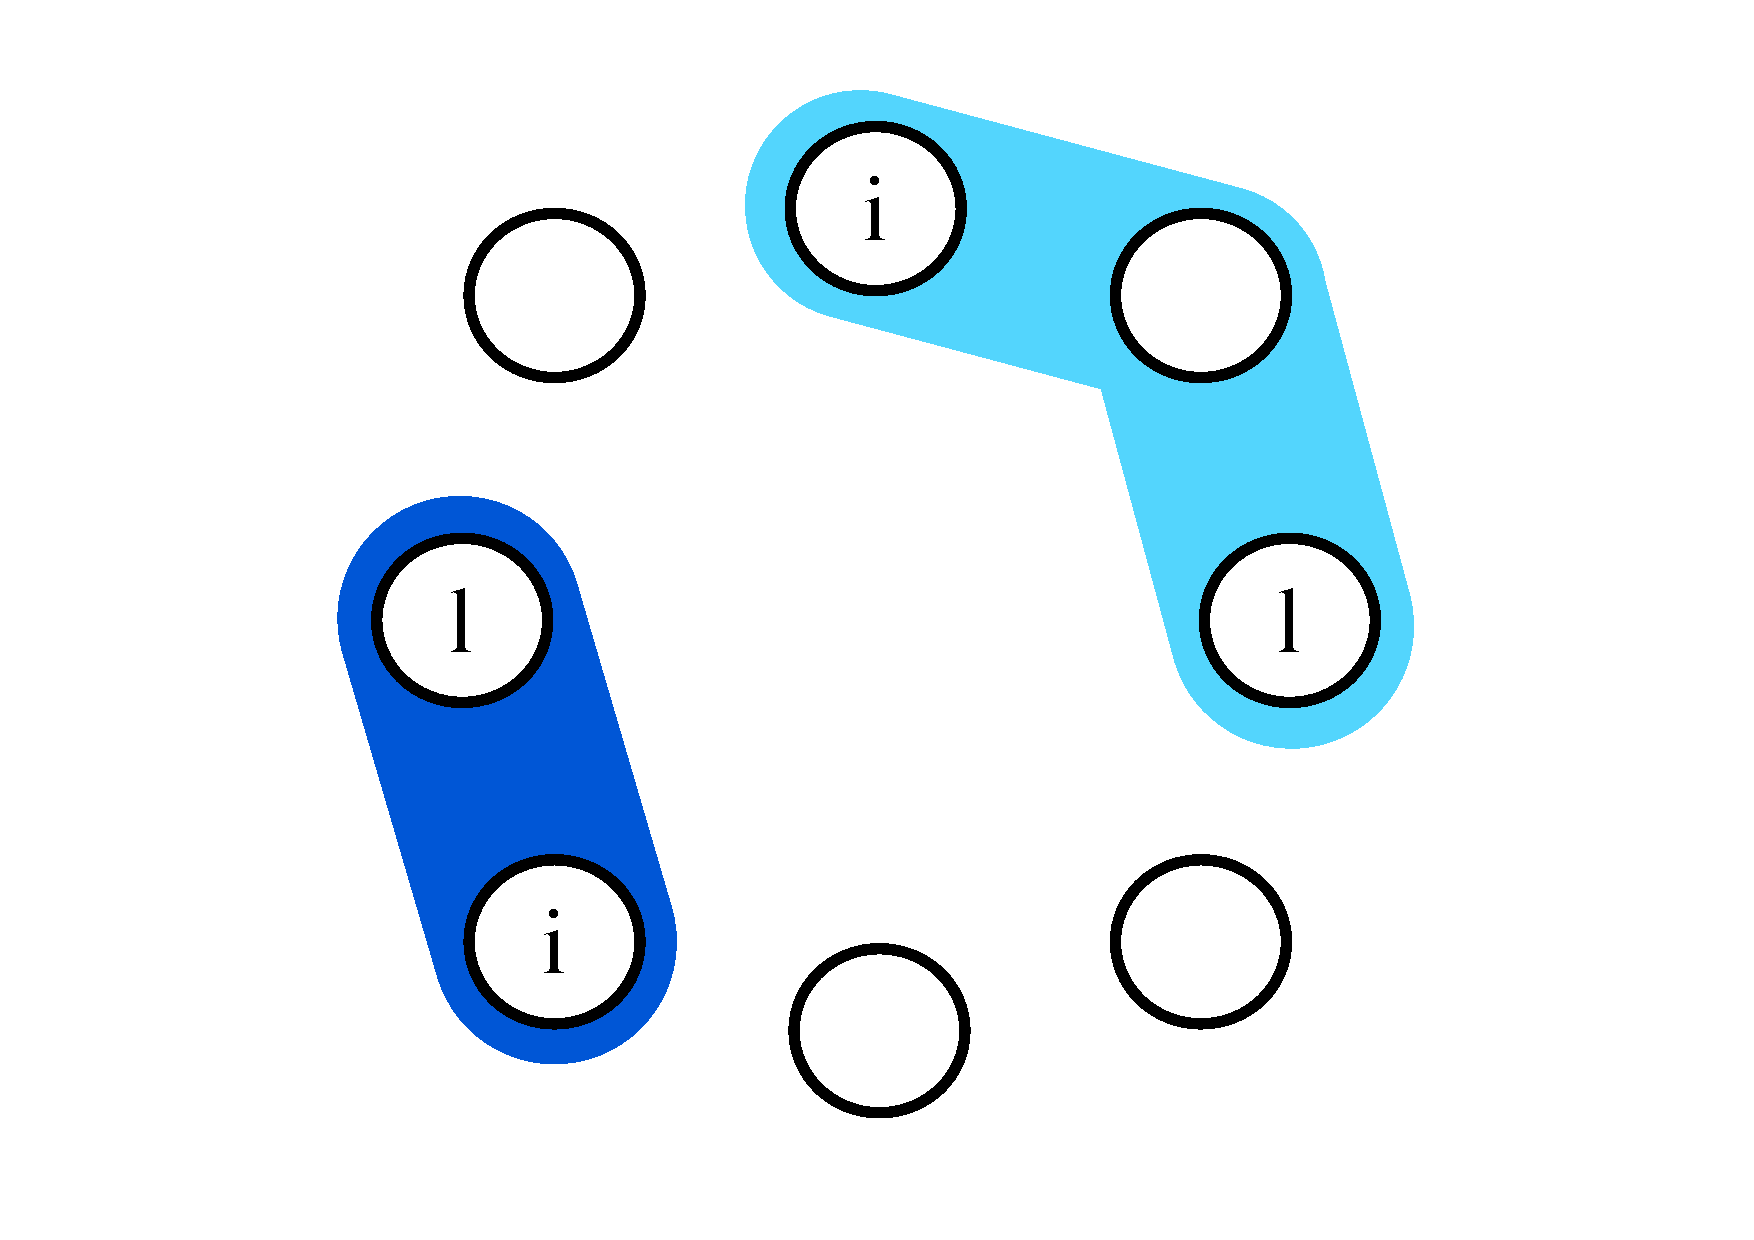
\includegraphics[width=2.7cm]{./figures/fig-26.pdf}
\label{fig:dvms_pte_3}}
%
\subfigure[Legend]{
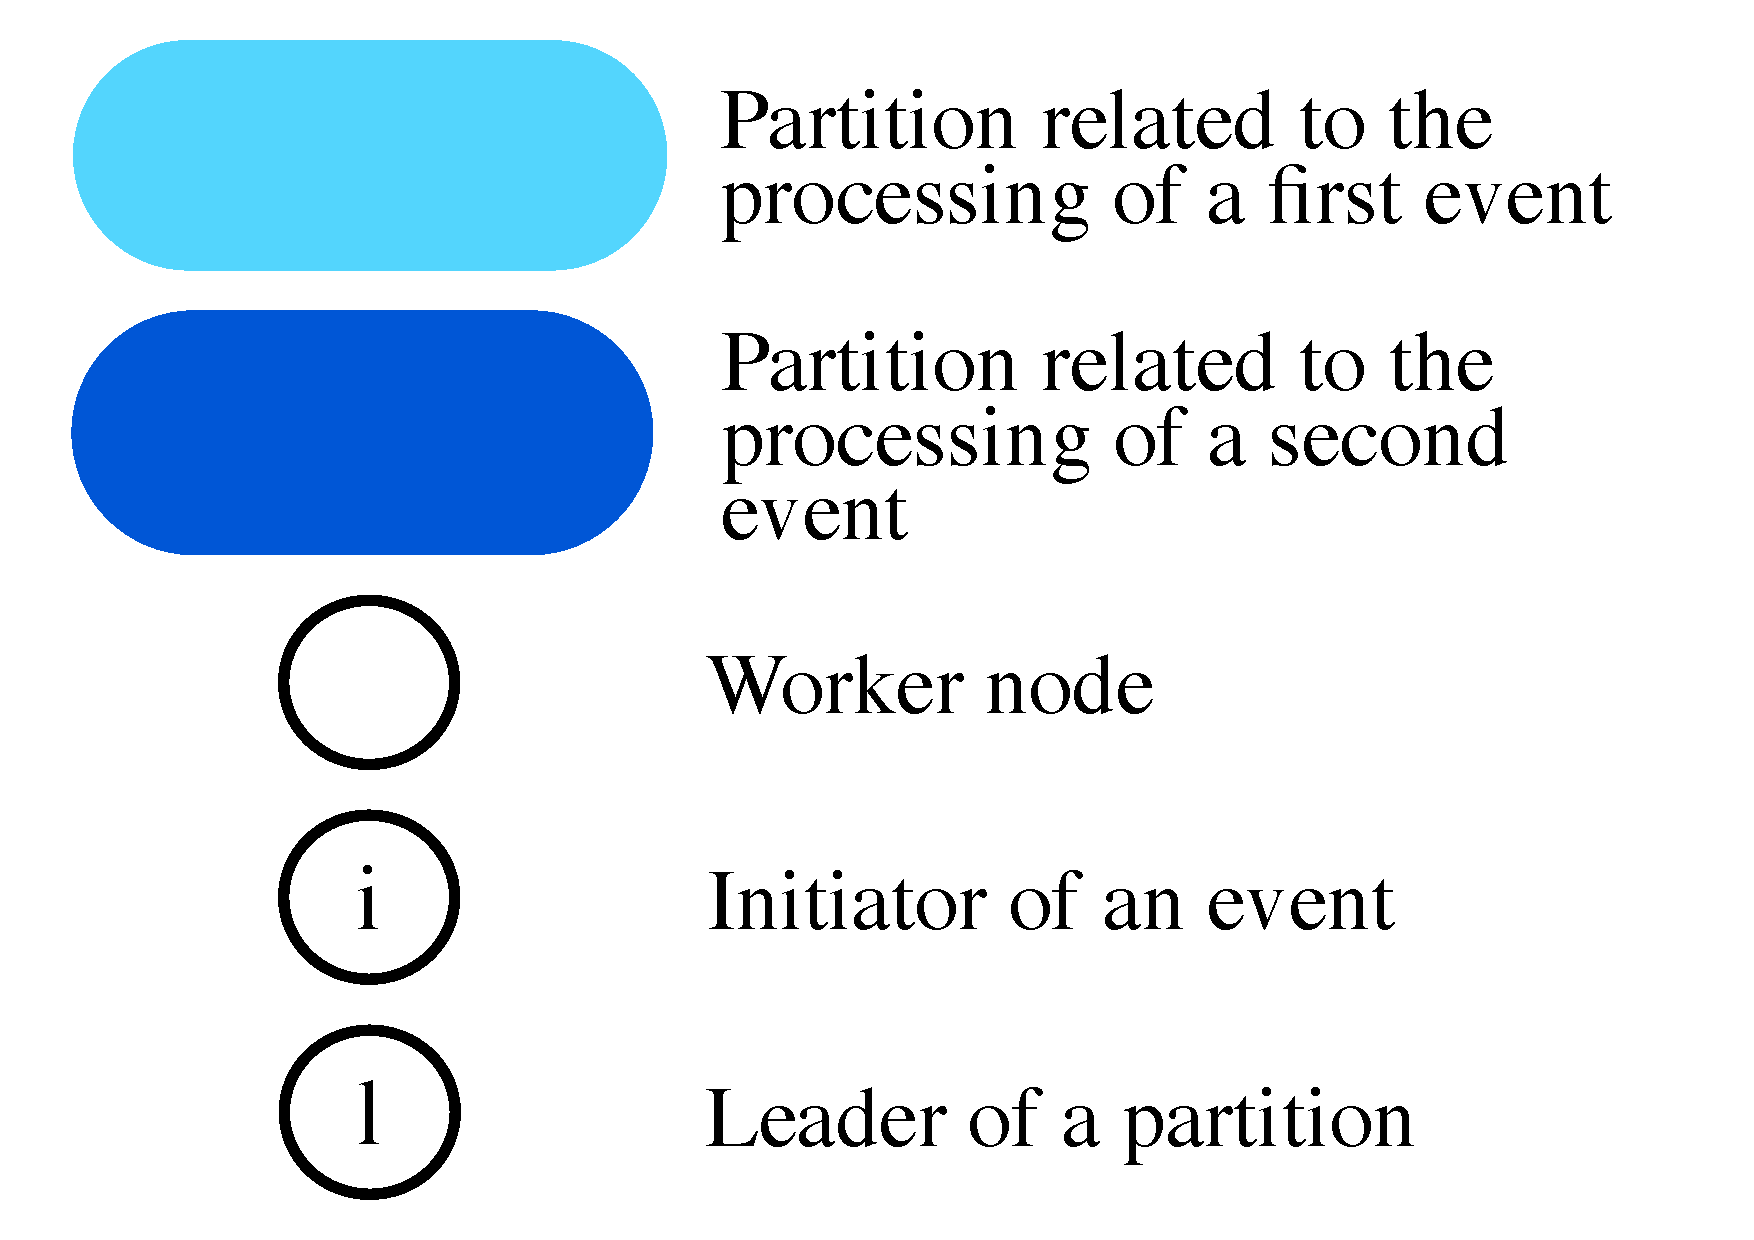
\includegraphics[width=2.7cm]{./figures/fig-27.pdf}
\label{fig:dvms_pte_4}}
%
\vspace*{-.3cm}
\caption{Processing two events simultaneously\label{fig:dvms_pte}}
\vspace*{-.6cm}
\end{figure}


% \subsubsection{Fault-tolerance}

% The main advantage of using overlay networks is that they have
% built-in fault tolerance mechanisms. DVMS therefore works on top of an
% overlay network such as Chord: when a node needs to rebalance its VMs
% workload, it uses the overlay network to find collaborators. For this
% study we implemented a simple overlay network as a flat list of
% agents: a typical request for collaborators includes the list of
% agents that are already collaborating with the requesting agent. A
% link to a new collaborator is then provided to the requesting
% agent. Communication is performed by message exchanges containing
% immutable data: our implementation harnesses the principles of the
% actor model in order to ease the handling of concurrency and
% distributed issues.

% Even if the implementation of the overlay network is simple, it
% fulfills its purpose, and in the case where one would want to use a
% different overlay network such as a ring topology, it only has to
% reuse the API provided by this simple implementation, and adapts its
% functionning to the targeted overlay network.
% \AL[JP]{here we do not describe DVMS in general but we should
% emphasize what has been exactly implemented and how} \JP[AL]{I added
% the preceding paragraph that gives more details about the overlay
% network used.}
%
% This functionning allows firstly a loosely coupling between DVMS and
% the overlay network used, and, secondly, to delegate most of the
% fault tolerance mechanisms to the overlay network. Although
% leveraging an overlay network to address node crashes is helpfull,
% it is not enough to make the problem solving procedure
% fault-tolerant.

% Harnessing the fault tolerance mechanisms of the underlying overlay
% network is, however, not sufficient. If the leader of a partition
% crashes, a new leader must take over in order for the resource problem
% to be solved and the nodes of a partition to be finally freed.  To
% avoid these issues, DVMS now relies on timeout mechanisms.  Each node
% of a partition periodically checks whether the state of its partition
% changed recently (\eg, if a new node joined the partition) and can
% thus identify if the partition's leader is not active anymore.  In
% this case, each node leaves the partition and can be integrated in
% other partitions.

%%% Local Variables:
%%% mode: latex
%%% TeX-master: "main"
%%% End:



%%% Local Variables:
%%% mode: latex
%%% TeX-master: "main"
%%% End:


\section{Experiments}
\label{sec:experiments}
%\AL[JP,AL,MS]{2 pages}
In this section, we, first, analyze the accuracy of \vmps by comparing
the  results of an Entropy execution through simulations and
\textit{in-vivo} experiments. This first experiment enables us to
confirm the expected behavior of \vmps Second, we present and discuss
our analysis of the three algorithms previously described.
We show that the performances of the hierarchical approach could
reached the distributed ones through minor changes.

%\subsection{Accuracy Evaluation of \vmps}
\subsubsection{Accuracy Evaluation}
\label{subsec:accuracy}
To validate the accuracy of \vmps, we implemented a dedicated
version of our
framework\footnote{\url{https://github.com/BeyondTheClouds/G5K-VMPlaceS}}
on top of the Grid'5000 testbed and compared the execution of the
Entropy strategy invoked every 60 seconds over a 3600 seconds period
in both the simulated and real world. Regarding the \textit{in-vivo}
conditions, experiments have been performed on top of the Graphene
cluster (Intel Xeon X3440-4 CPU cores, 16 GB memory, a GbE NIC, Linux
3.2, Qemu 1.5 and SFQ network policy enabled) with 6 VMs per node.
Each VM has been created as one of 8 VM predefined classes. The
template was 1:1GB:1Gbps:1Gbps:X, where the memory update speed X was
a value between 0 and 80\% of the migration bandwidth (1Gbps) in steps
of 10. Starting from 0\%, the load of each VM varied according to the
exponential and the Gaussian distributions previously described. The
parameters were $\lambda$ = Nb VMs/300 and $\mu$= 60, $\sigma$ = 20.
Concretely, the load of each VM varied on average every 5 min in steps
of 10 (with a significant part between 40\% and 80\%). A dedicated
\texttt{memtouch} program~\cite{Hirofuchi:2013:ALM:2568486.2568524} has
been used to stress both the CPU and the memory accordingly. Regarding
the simulated executions, \vmps has been configured to reflect the
\textit{in-vivo} conditions. In particular, we configured the network model of
SimGrid in order to cope with the network performance of the Graphene
servers that were allocated to our experiment (6 MBytes for the TCP
gamma parameter and 0.88 for the bandwidth corrective simulation
factor).
%\begin{figure}[hbt]
\begin{wrapfigure}{r}{.48\linewidth}
\centering
\vspace*{-.8cm}
%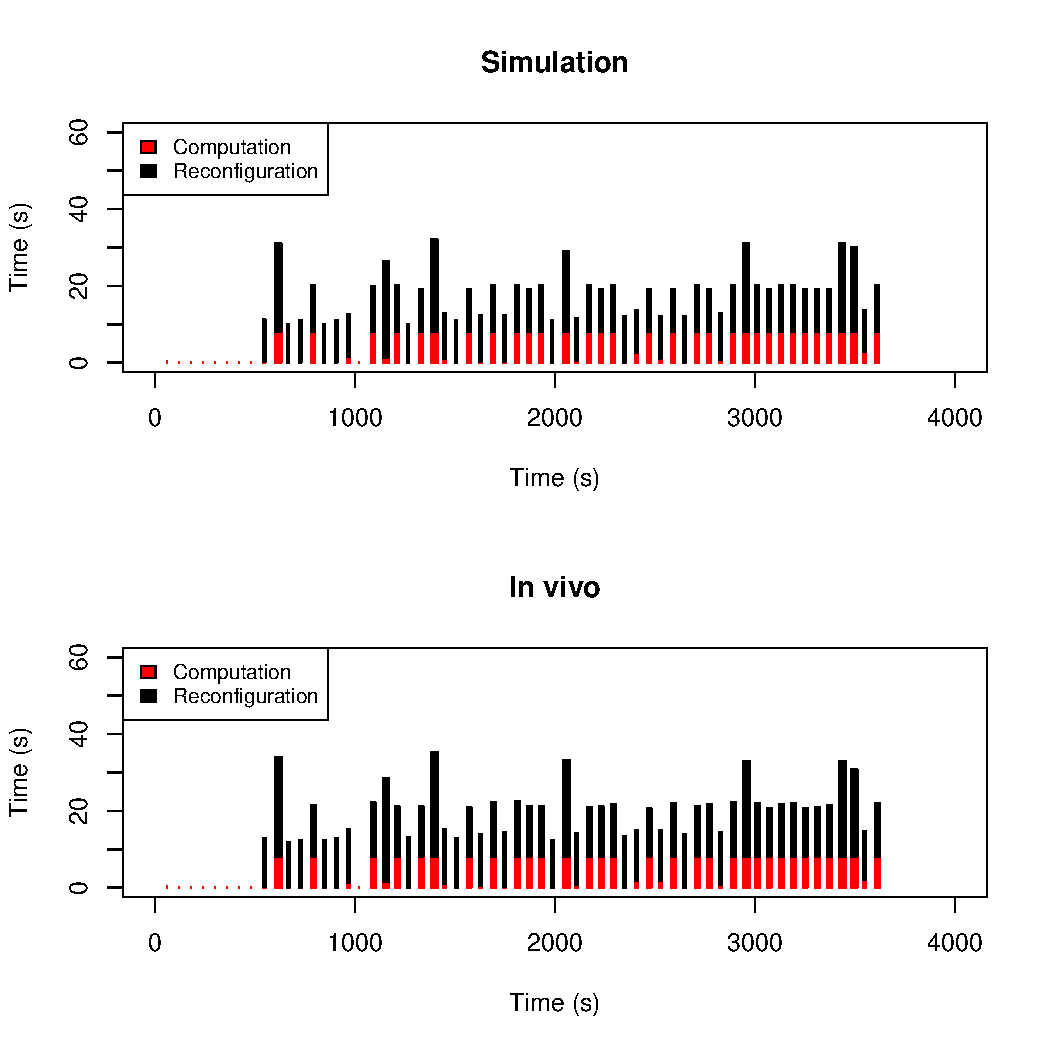
\includegraphics[width=0.99\linewidth]{./figures/simu-vivo-32PM-192VM-6020-original.pdf}
 \subcapcentertrue
\subfigure{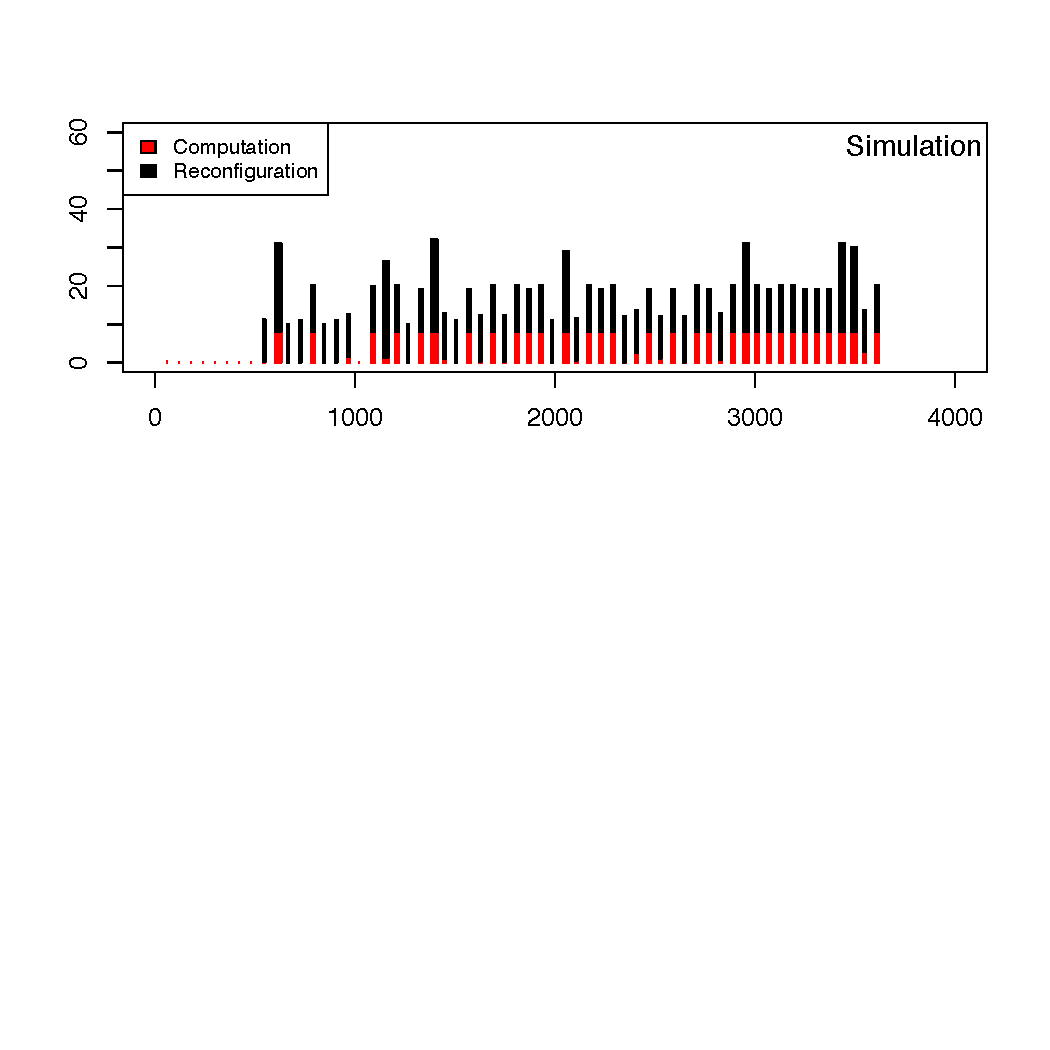
\includegraphics[width=0.99\linewidth]{./figures/accuraci-simu.pdf}
\label{fig:accu-simu}}
\subfigure{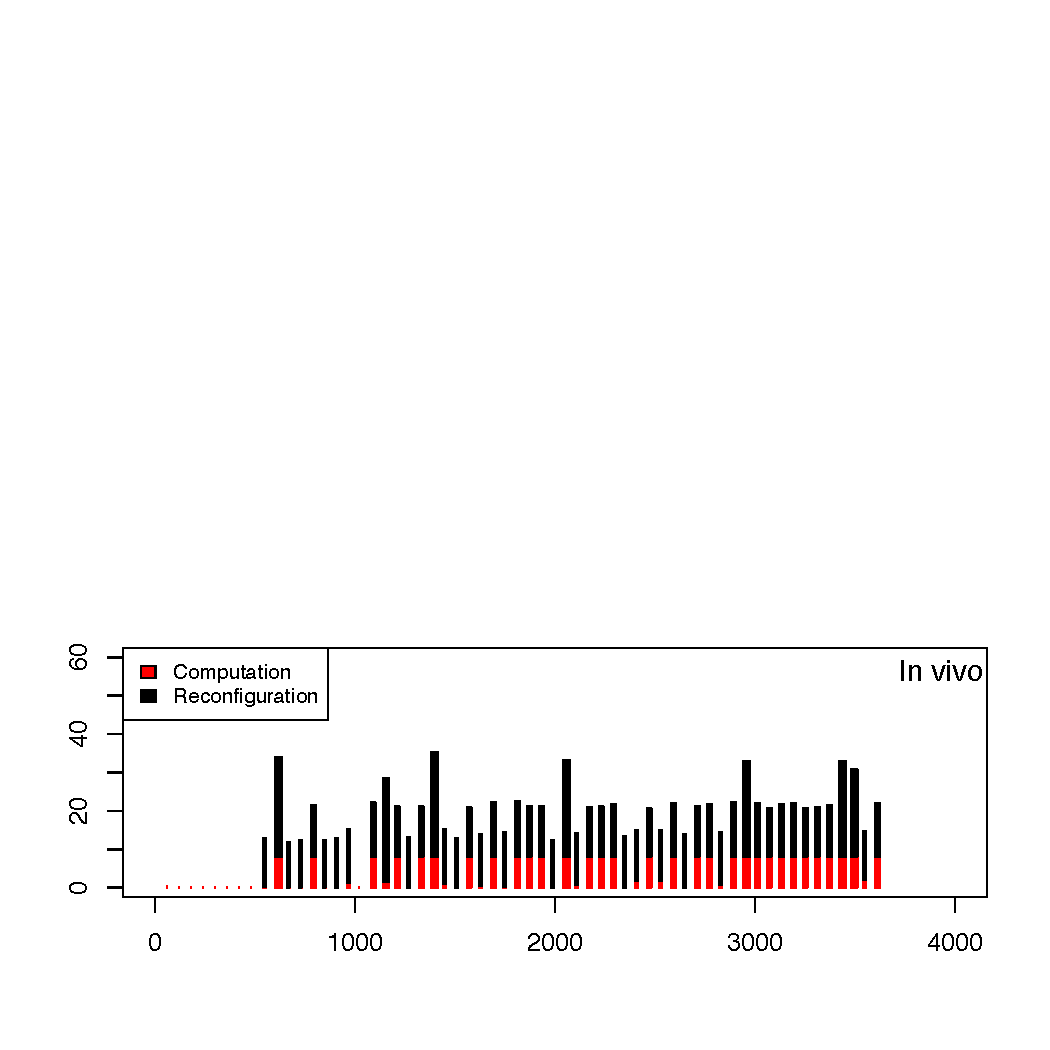
\includegraphics[width=0.99\linewidth]{./figures/accuraci-invivo.pdf}
\label{fig:accu-vivo}}
\vspace*{-.8cm}
\caption{Comparison between simulated (top) and \textit{in-vivo}
  (bottom) Executions}
\flushleft\scriptsize{The red parts correspond the computation phase (\ie
  the time where Entropy looks for a new configuration). The black parts correspond to the reconfiguration phase (\ie when
VM are relocated throughout the cluster.}
\label{fig:usecase-vivosimu}
\vspace*{-.6cm}
\end{wrapfigure}
%\end{figure}
Fig.~\ref{fig:usecase-vivosimu} shows the cost of the two phases of
the Entropy algorithm for each invocation when considering 32~PMs and
192~VMs through simulations (top) and in reality (bottom). At
coarse-grained, we can see that simulation results successfully
followed the in-vivo ones. During the first hundreds seconds, the cluster did not
experience VM requirement violations because the loads of VM were
still small (\ie Entropy simply validated that the curent placement
statisfied all VM requirements). At 540 seconds, Entropy started to
detect non viable configurations and performed reconfigurations.
Diving into details, the difference between the \textit{simulated} and
\textit{in-vivo} reconfiguration time fluctuated between 6\% and 18\%
(median was around 12\%). %during the experiment.
The worst case, \ie 18\%, was reached when
multiple migrations were performed simultaneously on the same
destination node. In this case and even if the SFQ network policy was
enabled, we discovered that in the reality the throughput of migration
traffic fluctuated when multiple migration sessions simultaneously
shared the same destination node. We confirmed this point by analyzing
TCP bandwidth sharing through \texttt{iperf} executions. We are
currently investigating with the \sg core-developpers how we can
integrate this phenomenon into the live-migration model. Howver, as a
migration lasts less than 15 seconds in average, we believe that that
the current simulation results are sufficiently accurate to capture
performance trends of placement strategies.


% As an example, we noticed that applying the
% reconfiguration plan was much more time-consuming than computing it. This result that has been correctly reported by the simuations means that VMPP also needs
% to address the way of shorten reconfiguration phases, not only that of
% computing ones.
% % This is rather important as most relocation
% % algorithms try to reduce the computation phase instead of focusing on the
% % reconfiguration one.
% Leveraging \vmps will enable researchers to observe such key points
% without facing with the burden of conducting large scale
% \textit{in-vivo} experiments. We illustrate such an advantage in the
% following section.

%\subsection{A First Use-Case:  Comparison of Entropy, Snooze and DVMS}
\subsubsection{Analysis of Entropy, Snooze and DVMS}
\label{subsec:first-usecase}
%\AL{Il faudra parler du nombre de migrations qui est egalement une
%  métrique pertinente. Plusieurs algorithms tentent de reduire cette
%  metrique }
%\AL[AL]{Il faudra mettre des snapshots de PajeNG}
% Evaluation of VMPlaceS on Grid'5000: simulations were running on one server.
In this paragraph, we discuss the results of the simulations we
performed on the Entropy,  Snooze and DVMS strategies.
% Due to space limitations we present a generaly study
% analyzing the violation times as well as the
% duration of the computation and reconfiguration phases. However, we
% highlight that such a study enables us to investigate some variant and possible
% improvements of Snooze and DVMS that made possible to easily study  thanks to
% \vmps.

%\subsubsection{Experimental Conditions}
Regarding the experimental conditions, all simulations have been
performed on the Lyon clusters of the Grid'5000 testbed.
Each execution was running on a dedicated server, thus avoiding
interferences between simulations and ensuring reproducibility between
the different invocations.
% Scripts: automation of the deployment, running of simulations and the collect
% of results.
% It enables us to run a large number of simulations, with several variants
% of the scheduling algorithm.
%
\vmps has been configured to simulate an homogeneous
infrastructure of PMs composed of 8 cores, 32~GB of RAM and 1~Gpbs
Ethernet NIC. To enable fair comparison between the three strategies,
the scheduling resolver only considered 7 cores (\ie one was devoted
to run the Snooze LC or the DVMS processes). Dedicating one core for
the host OS and other administrative processes is something which is
rather usual and thus we believe acceptable in our experimental
methodology.  Ten VMs have been
initially launched on each simulated PM. Each VM relied one of the VM
classes described in the accuracy experiment and the
parameters for changing the load were the same ($\lambda$ = Nb
VMs/300, $\mu$ = 60 and $\sigma$ = 20). The stationary state was
reached after 20 min of the simulated time with a global cluster load
of 85\%.
%as depicted in Fig. \ref{fig:load_figure}.
To accelerate the simulations, we have chosen to limit the simulated time to 1800
seconds. It is noteworthy that the consolidation ratio, \ie the number
of VMs per node, has been defined to generate a sufficient number of
violations. We discovered that under a global load of 75\%, our
infrastructure almost did not face VM violations with our selected Gaussian
distribution. Such a result is rather
satisfactory as it can explained why most production DCs target such
an overall utilization rate.\footnote{\url{http://www.cloudscaling.com/blog/cloud-computing/amazons-ec2-generating-220m-annually/}}
Finally, infrastructures composed of
128, 256, 512 and 1024 PMs, hosting respectively 1280, 2560, 5120 and
10240 VMs have been investigated. For Entropy and Snooze that rely on
service nodes, additional simulated PMs have been provided. For Snooze, one GM
has been created every 32 LCs (\ie PMs). The frequency to invoke the
solver has been setted to 30 seconds for Entropy and the Snooze GMs.
We remind that no service
node had to be provisioned for DVMS as a DVMS process has been
executed directly on top of each hosting node.
%
% In order to cope with real DC conditions, we defined the parameters
% for node crashes to simulate a fault on average every 6 months for a
% duration of 300 seconds. These values correspond to the Mean Time To
% Failure (MTTF) and the Mean Time To Repair (MTTR) of a Google DC
% server~\cite[pp. 107-108]{datacenterAsComputer}. We underline that at
% the scale we performed our simulations such a crash ratio was not
% sufficient to impact the behavior of the scheduling policies.
% Dedicated simulations were mandatory to study the influence of node
% crashes. However, due to the space limitations, we do not present them
% in the article and only gives major trends. Regarding Entropy,
% although the lost of the service node can be critic, the failure
% probability is so small that the single point of failure issue can be
% easily solved by a fail-over approach. Regarding Snooze, the heartbeat
% strategy enables the reconstruction of the hierarchy in a relative
% short time and thus crashes on service nodes do not significantly
% impact the resolution of violations (in our case less than 10 seconds
% is mandatory to reorganize the Snooze topology with a 6 seconds
% heartbeat mechanism). Finally regarding DVMS, the crash of one node
% does not have any impact of the resolution has the composition of the
% microcosm is reevaluated immediately.
%%
%Finally, we highlight that all configuration files used to perform the discussed simulations can
%be downloaded from the \vmps repository.

%\subsubsection{General  Analysis}
%\label{subsec:general-comparison}

% \begin{figure}
% \subcapcentertrue
% \subfigure[Infrastructure load]{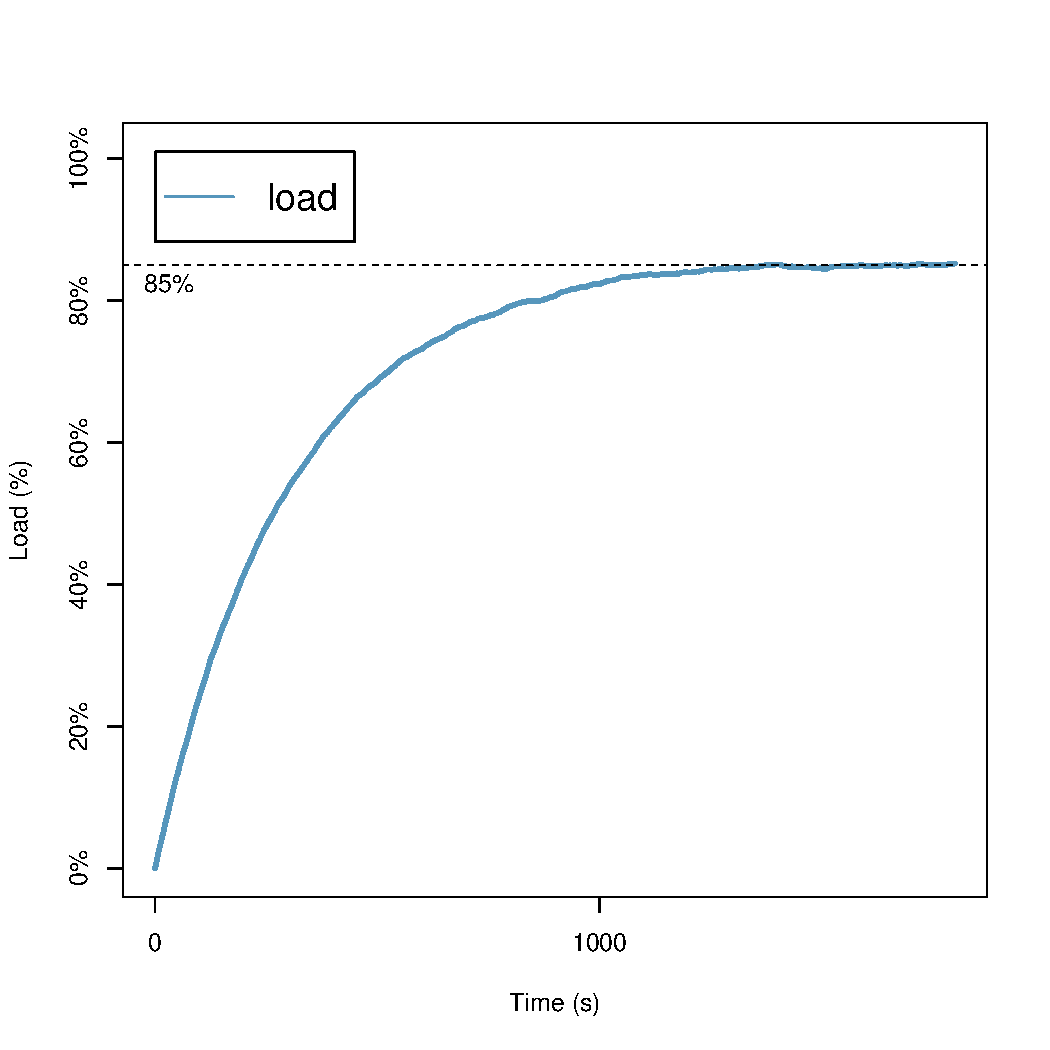
\includegraphics[width=4cm]{./figures/experiments/1024-hierarchical.pdf}\label{fig:load_figure}}
% \subfigure[Cumulated Violation Time]{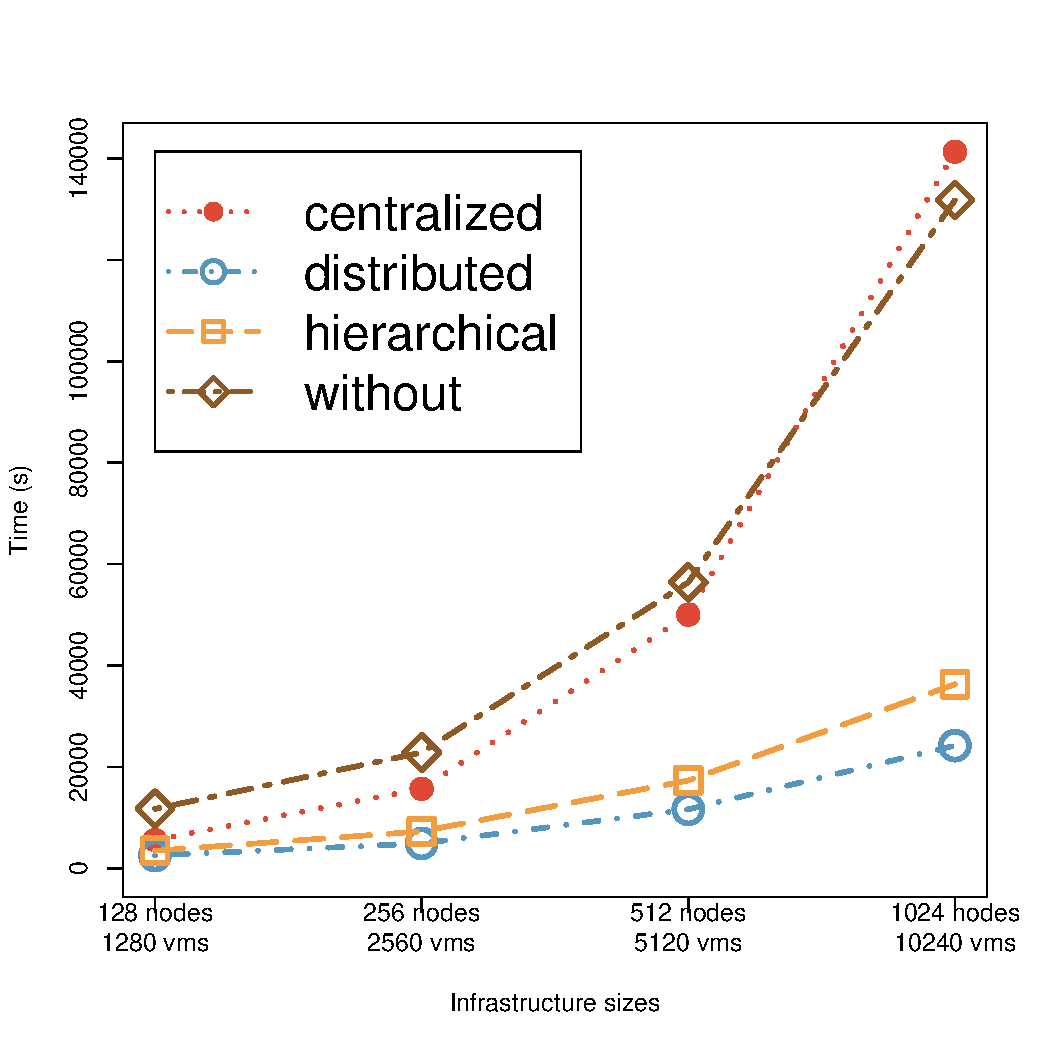
\includegraphics[width=4cm]{./figures/experiments/violation_time.pdf}\label{fig:cumulated_violation}}
% \caption{Simulation Results - 10 VMs per node (VM load: $\mu=60$ and $\sigma=20$)}
% \label{fig:simulation-overview}
% \end{figure}

\begin{figure*}
\subcapcentertrue
\subfigure{
  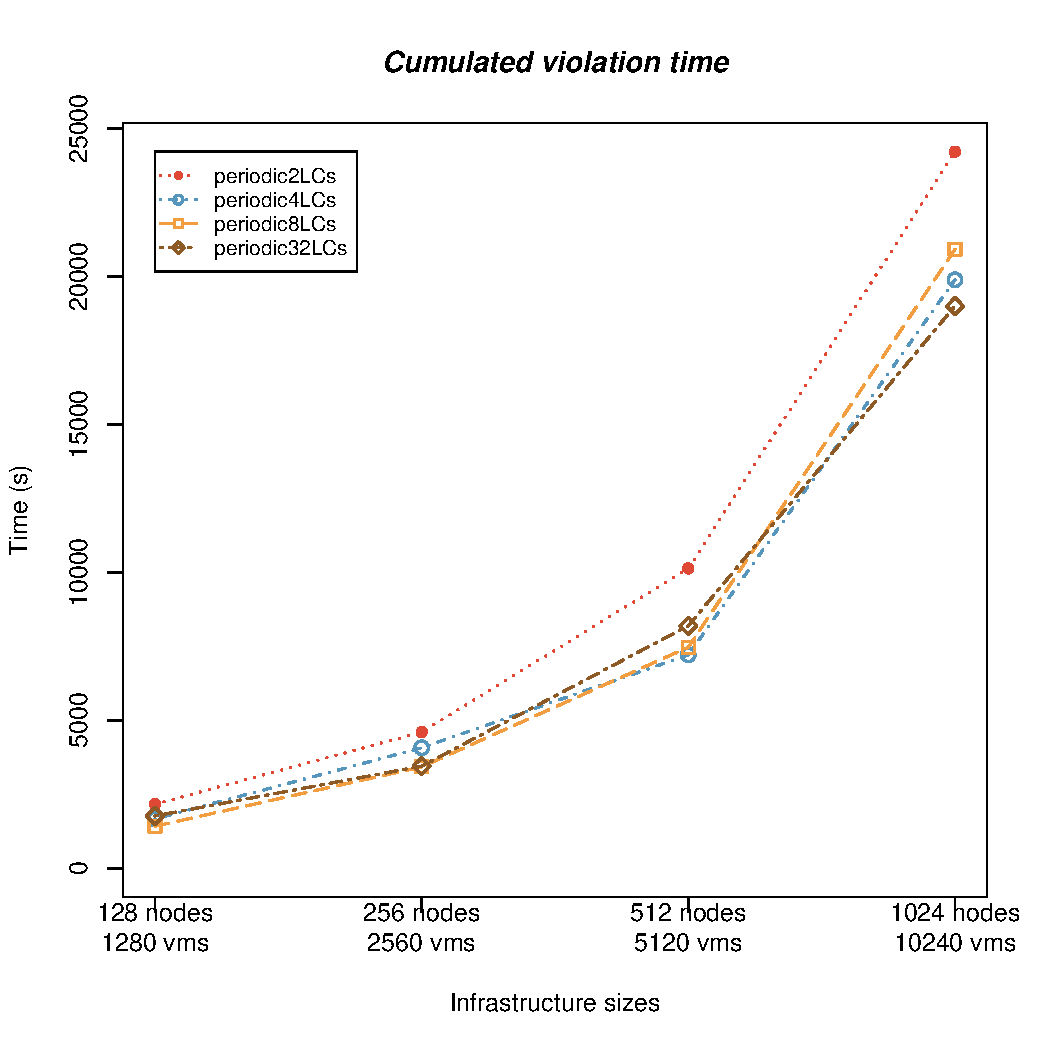
\includegraphics[width=.46\textwidth]{figures/groupSizes-violationTime.pdf}
  \label{fig:groupSizesViolationTime}}
\begin{minipage}{.5\textwidth}
\centering
  \vspace*{-6cm}
%\subfigure[Duration of violation ($med \pm \sigma$)]{
\subfigure{
    {\tiny \begin{tabular}{|P{17mm}@{\:}||@{\:}c@{\:}|@{\:}c@{\:}|@{\:}c@{\:}|}
      \thickhline
      \textbf{Infrastructure size}
        & \multicolumn{3}{c@{\:}|}{\textbf{Duration of violations}
          ($med \pm \sigma$)}
          \Tstrut \\
         \hfill  & ~Centralized~ & ~Hierarchical~ & Distributed \Bstrut \\
      \thickhline
        128 nodes   & 21.26 $\pm$ 13.55 & 21.07 $\pm$ 12.32 &   9.55 $\pm$ 2.57 \\
        256 nodes   & 40.09 $\pm$ 24.15 & 21.45 $\pm$ 12.10 &   9.58 $\pm$ 2.51 \\
        512 nodes   & 55.63 $\pm$ 42.26 & 24.54 $\pm$ 16.95 &   9.57 $\pm$ 2.67 \\
        1024 nodes  & 81.57 $\pm$ 86.59 & 29.01 $\pm$ 38.14 & \:9.61 $\pm$ 2.54
      \Rstrut  \\ \hline
      \thickhline
  \end{tabular} }
%\label{table:detailed_violation_time}
}
  \vspace*{-.2cm}

%\subfigure[Duration of computations ($Med \pm \sigma$)]{
\subfigure{
    {\tiny \begin{tabular}{|P{17mm}@{\:}||@{\:}c@{\:}|@{\:}c@{\:}|@{\:}c@{\:}|}
      \thickhline
      \textbf{Infrastructure size}
        & \multicolumn{3}{c@{\:}|}{\textbf{Duration of computations}
          ($med \pm \sigma$)}
          \Tstrut \\
         \hfill  & ~Centralized~ & ~Hierarchical~ & Distributed \Bstrut \\
      \thickhline
        128 nodes   &  3.76 $\pm$  7.43 &  2.52 $\pm$  4.63 &   0.29 $\pm$ 0.03 \\
        256 nodes   &  7.97 $\pm$ 15.03 &  2.65 $\pm$  4.69 &   0.25 $\pm$ 0.02 \\
        512 nodes   & 15.71 $\pm$ 29.14 &  2.83 $\pm$  4.98 &   0.21 $\pm$ 0.01 \\
        1024 nodes  & 26.41 $\pm$ 50.35 &  2.69 $\pm$  4.92 & \:0.14 $\pm$ 0.01
      \Rstrut  \\ \hline
      \thickhline
  \end{tabular} }
%\label{table:detailed_computation_time}
}
  \vspace*{-.2cm}

%\subfigure[Duration of reconfigurations ($Med \pm \sigma$)]{
\subfigure{
    {\tiny \begin{tabular}{|P{17mm}@{\:}||@{\:}c@{\:}|@{\:}c@{\:}|@{\:}c@{\:}|}
      \thickhline
      \textbf{Infrastructure size}
        & \multicolumn{3}{c@{\:}|}{\textbf{Duration of  reconfigurations}
          ($med \pm \sigma$)}
          \Tstrut \\
         \hfill  & ~Centralized~ & ~Hierarchical~ & Distributed \Bstrut \\
      \thickhline
        128 nodes   & 10.34 $\pm$  1.70 &  10.02 $\pm$  0.14 &   10.01 $\pm$ 0.11 \\
        256 nodes   & 10.26 $\pm$  1.45 &  10.11 $\pm$  0.83 &   10.01 $\pm$ 0.08 \\
        512 nodes   & 11.11 $\pm$  3.23 &  10.28 $\pm$  1.50 &   10.08 $\pm$ 0.82 \\
        1024 nodes  & 18.90 $\pm$  7.57 &  10.30 $\pm$  1.60 & \:10.04 $\pm$ 0.63
      \Rstrut  \\ \hline
      \thickhline
  \end{tabular} }
%\label{tab:detailed_reconf_time}
}
\end{minipage}
\vspace*{-.6cm}
\caption{Scalability/Reactivity analysis of Entropy, Snooze and DVMS}
\label{fig:general-comparison}
\vspace*{-.8cm}
\end{figure*}

Fig.~\ref{fig:general-comparison} presents on the left the cumulated violation
time for each placement policy and on the right several tables that give more details by presenting the
mean and the standard deviations of the duration of, respectively, the
violations and the computation/reconfiguration phases. As
anticipated, the centralized approach did not scale and became almost
counterproductive for the largest scenario in comparison to a system
that did not use any dynamic scheduling strategy. The more nodes Entropy has to
monitor, the less efficient it is on both the computation and
reconfiguration phases. Regarding the computation, the VMPP is a
NP-Hard problem and thus it is not surprising that it takes more time
to resolve larger problems. Regarding the reconfiguration, as Entropy
has to solve much more violations simultaneously, the reconfiguration plan
is more complex for large scenarios, including several migrations
coming from and going to the same nodes. Such reconfiguration plans
are non optimal as they increase the bottleneck effects at the network
level of each involved PM. Such a simulated result is valuable as it confirms
that reconfiguration plans should avoid as much as possible such
manipulations.
%
Regarding Snooze, although the performances are better than the
Entropy ones, we may erroneously conclude that the hierarchical
approach is not competitive with respect to the distribued strategy at
the first sight. However, diving into details, we can see that both
the computation and reconfiguration phases are almost constants
(around 3 seconds and 10 seconds) and not so far from the DVMS values,
especially for the reconfiguration phase, which is predominant. These
results can be easily explained: the centralized policy adresses the
VMPP by considering all nodes at each invovation, while the
hierarchical and the distributed algorithms divide the VMPP into sub
problems, considering smaller numbers of nodes (32~PMs in Snooze and
4 in average with DVMS). To clarify the influence of the group size on
the Snooze performances, \ie the ratio of LCs attached to one GM, we
performed additional simulations aiming at investigating whether a
smaller group size can lead to similar performances of DVMS. We
higlight that the use of \vmps eased such a study as it has consisted
to simply relaunch the previous simulation with a distinct
assignment.


\begin{figure*}
  \vspace*{-.5cm}
\subcapcentertrue
%\subfigure[Total Violation Times]{
\subfigure{
  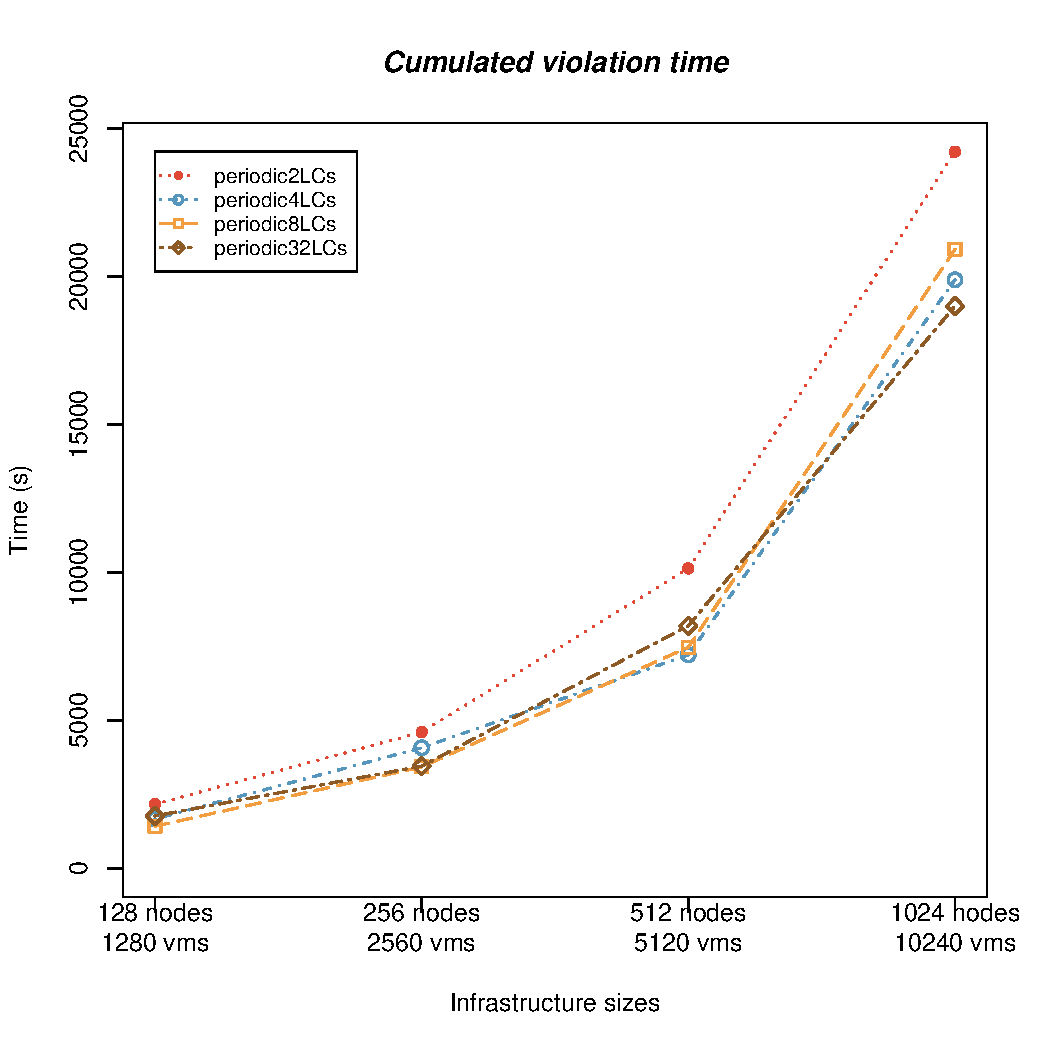
\includegraphics[width=.38\textwidth]{figures/groupSizes-violationTime.pdf}
  \label{fig:groupSizesViolationTime}}
\begin{minipage}{.60\textwidth}\centering
  \vspace*{-4.5cm}
%\subfigure[No.\ of Failed Reconfigurations]{
\subfigure{
    {\tiny \begin{tabular}[b]{|r@{\:}||@{\:}r@{\:}|@{\:}r@{\:}|@{\:}r@{\:}|@{\:}r@{\:}|}
      \thickhline
      \textbf{Infra.\ Size~~}
        & \multicolumn{ 4 }{c@{\:}|}{\textbf{No.\ of failed reconfigurations}}
          \Tstrut \\
         \hfill &  ~2 LCs~ & ~4 LCs~ & ~8 LCs~ &  ~32 LCs~  \Bstrut \\
      \thickhline

        128~~~~~~~ &  19~ & 0~ & 0~ & 0~ \\
        256~~~~~~~ &  29~ & 0~ & 0~ & 0~ \\
        512~~~~~~~ &  83~ & 1~ & 0~ & 0~ \\
       1024~~~~~~~ & 173~ & 7~ & 0~ &  0
      \Rstrut  \\ \hline
      \thickhline
  \end{tabular} }
  \label{fig:groupSizesReconfigFail}
  }
\vspace*{-.2cm}

%\subfigure[Means $\pm$ Std deviations of computation durations.]{
\subfigure{
    {\tiny \begin{tabular}[b]{|r@{\:}||@{\:}c@{\:}|@{\:}c@{\:}|@{\:}c@{\:}|@{\:}c@{\:}|}
      \thickhline
      \textbf{Infra.\ Size~~}
        & \multicolumn{ 4 }{c@{\:}|}{\textbf{Duration of the
            computations $(Med \pm \sigma)$}}
          \Tstrut \\
         \hfill &  ~2 LCs~ & ~4 LCs~ & ~8 LCs~ & 32 LCs  \Bstrut \\
      \thickhline

        128~~~~~~~ &   0.16 $\pm$   1.23 &   0.34 $\pm$   1.81 &   0.58 $\pm$   2.40 &   2.53 $\pm$   4.62  \\
        256~~~~~~~ &   0.18 $\pm$   1.31 &   0.42 $\pm$   1.99 &   0.66 $\pm$   2.50 &   2.65 $\pm$   4.69  \\
        512~~~~~~~ &   0.15 $\pm$   1.20 &   0.33 $\pm$   1.78 &   0.67 $\pm$   2.54 &   2.83 $\pm$   4.98  \\
       1024~~~~~~~ &   0.19 $\pm$   1.37 &   0.42 $\pm$   2.02 &   0.89 $\pm$   2.90 &   ~2.69 $\pm$   4.91

      \Rstrut  \\ \hline
      \thickhline
  \end{tabular} }
  \label{fig:groupSizesComputationTime}
  }
\end{minipage}
\vspace*{-.6cm}
\caption{Hierarchical placement: influence of varying group sizes}
\label{fig:snoozeGroupSizes}
\vspace*{-.6cm}
\end{figure*}
%
%\paragraph{Varying group sizes}
%
Figure \ref{fig:snoozeGroupSizes} presents the simulated values
obtained for scenarios with 2,~4,~8 and 32~LCs per GM for four
infrastructure sizes. The overall performance (\ie cumulated violation
time) shows that
2~LCs per GM result in significantly higher violation times.
% All other
%group sizes yield violation times that are relatively close, which
%indicates that a small group size does not help much in
%resolving violations faster.
The relatively bad performance of the smallest group size can be
explained in terms of the number of failures of the reconfiguration
process, that is, overloading situations that are discovered but
cannot be resolved because the GM managing the overloaded VM(s) did
not dispose of enough resources (see tables on the right).
Groups of 2~LCs per GM are clearly insufficient at our global load level (85\%).
Failed reconfigurations are, however, already very rare in the case of
4~LCs per GM and do not occur at all for 8~and 32~LCs per GM. This is
understandable because the load is statistically evenly distributed
among the LCs and tthe load profile we evaluated only rarely results
in many LCs of a GM to be overloaded. Violations can therefore be
resolved even in the case of a smaller number (4) LCs available for
load distribution.
Conversely, we can see that the duration of the computation phases
decreases strongly along with the group
size. It reaches a value close to the computation times of DVMS for a
group size of 4-LCs per GM.% see Fig.~\ref{fig:groupSizesComputationTime}.
We thus cannot minimize computation times and violation times by
reducing the number of LCs because larger group sizes are necessary to
resolve overload situations if the VM load gets higher.
In contrast, DVMS resolves this trade-off by construction because of its
automatic and dynamic choice of the partition size necessary to handle
an overload situation.
Once again,
this information is valuable as it will help researchers to design new
algorithms favoring the automatic discovery of the optimal subset of
nodes capable to solve violations under for given load profiles.
% Although DVMS selects naively its neighborhood without
% considering whether it is relevant or note, we can consider that DVMS
% is one of such advanced algorithm.


% \begin{figure}[ht]
% \begin{center}
%     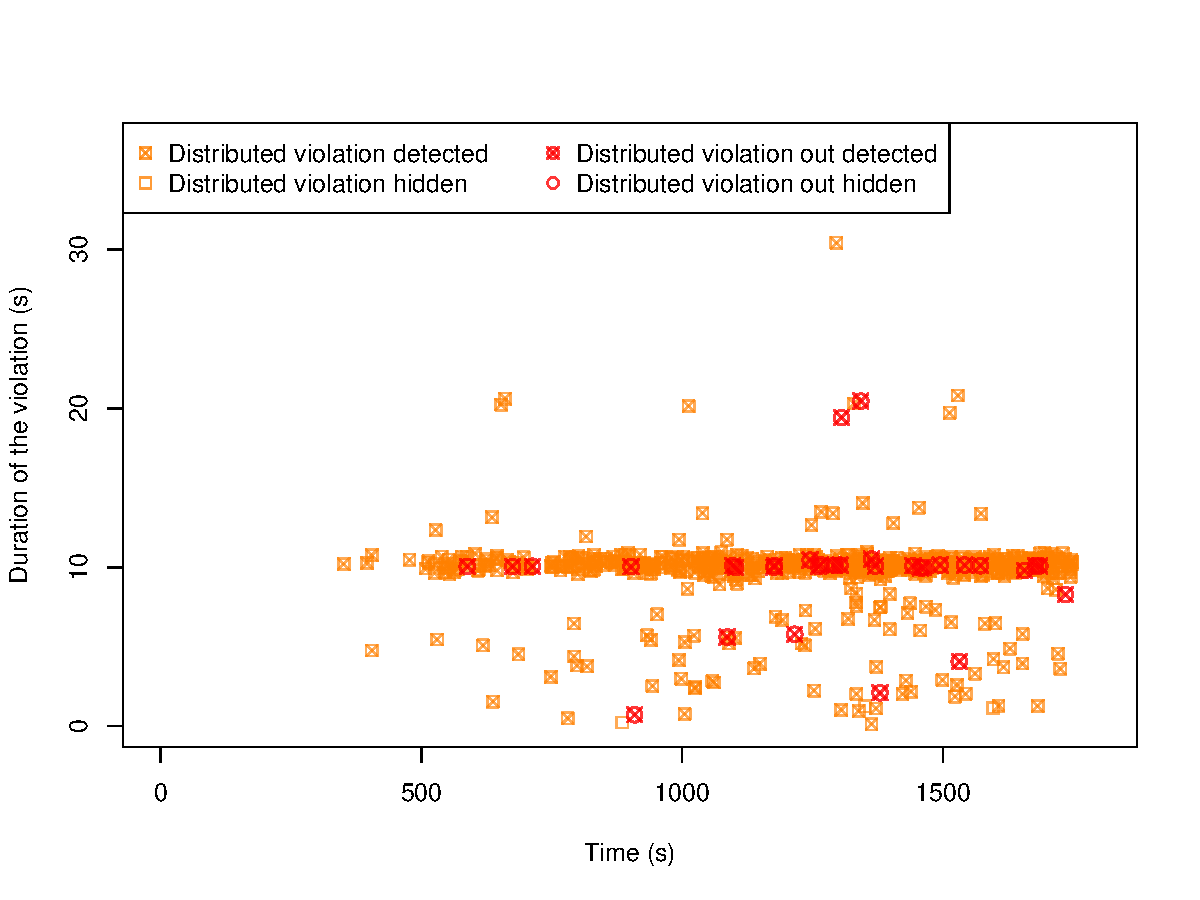
\includegraphics[width=.85\linewidth]{figures/experiments/clouds-1024-distributed.pdf}
%     \caption{Details of violations duration occuring during simulation (10240 VMS).}
% \end{center}
% \label{fig:violation_clouds_dvms_1024}
% \end{figure}

% \begin{figure}[ht]
% \begin{center}
%     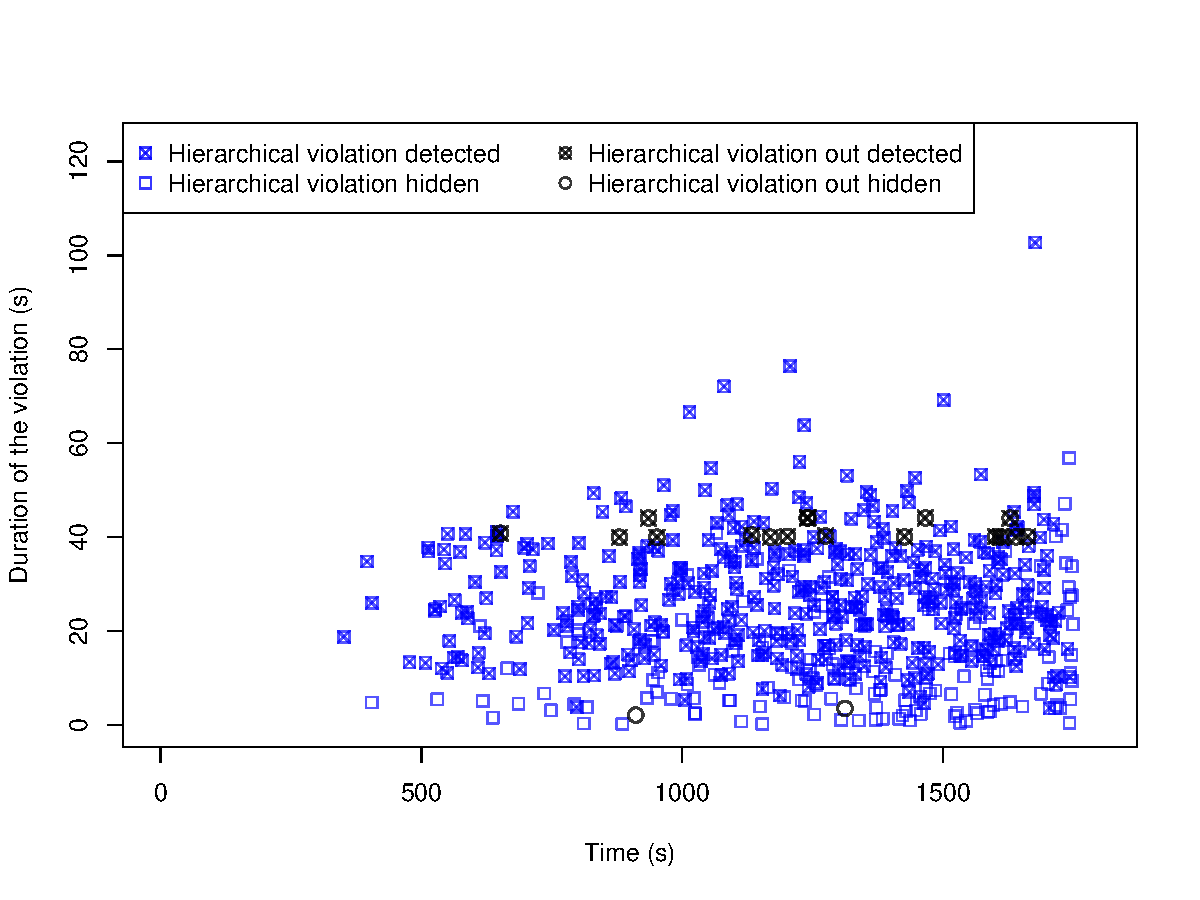
\includegraphics[width=.85\linewidth]{figures/experiments/clouds-1024-hierarchical.pdf}
%     \caption{Details of violations duration occuring during simulation (10240 VMS).}
% \end{center}
% \label{fig:violation_clouds_snooze_1024}
% \end{figure}


\begin{figure}[ht]
\begin{center}
    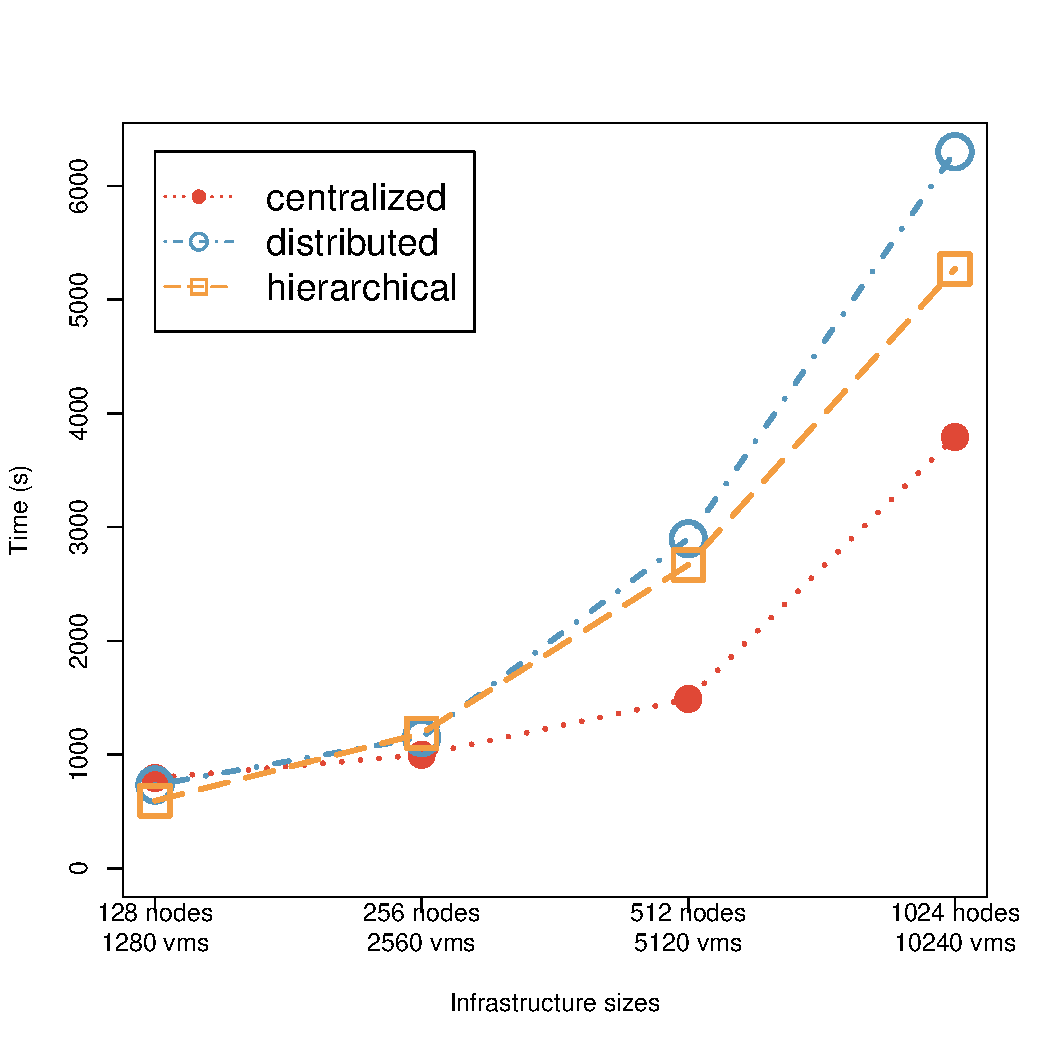
\includegraphics[width=.65\linewidth]{figures/experiments/migration_time.pdf}
    \caption{Cumulated migration time.}
\end{center}
\label{fig:cumulated_migration_time}
\end{figure}

\begin{figure}[ht]
\begin{center}
    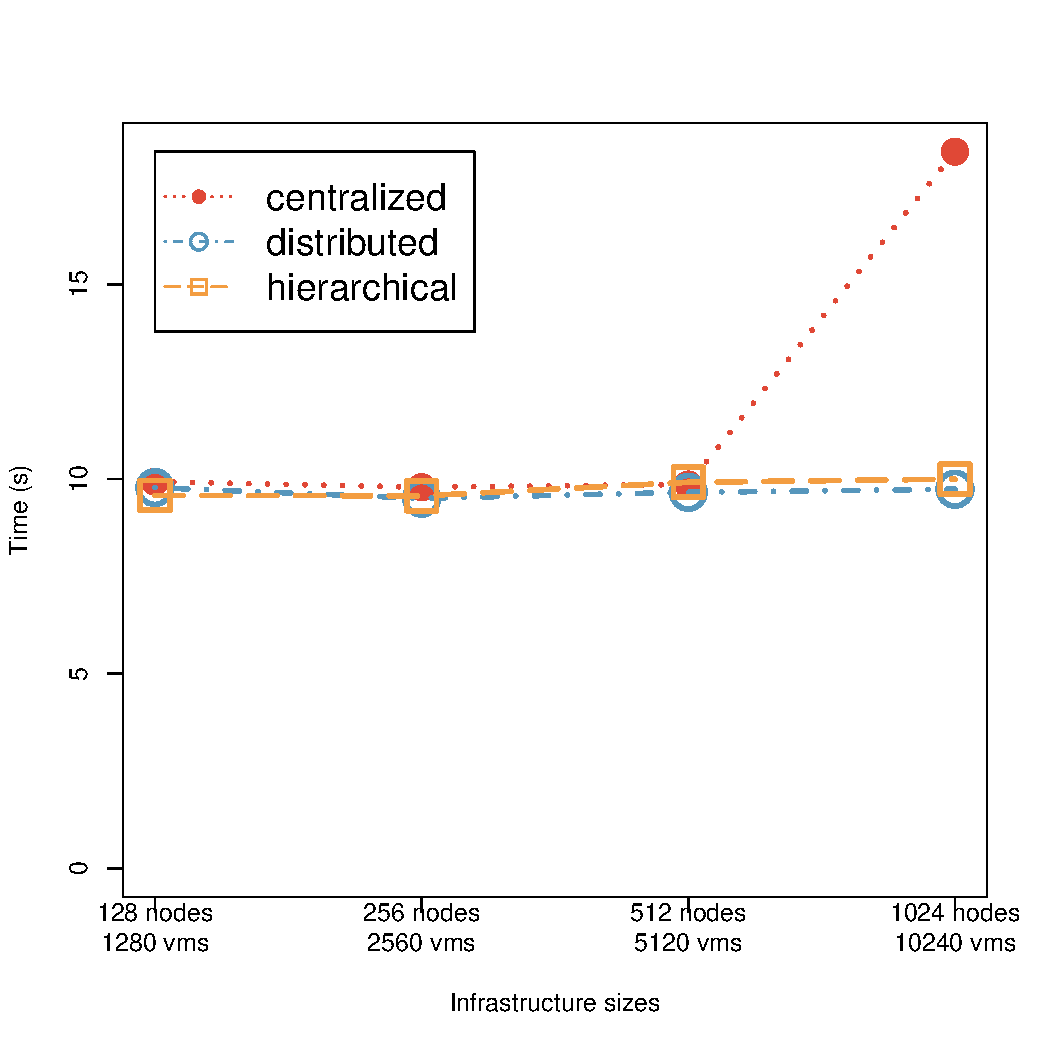
\includegraphics[width=.65\linewidth]{figures/experiments/migration_avg_duration.pdf}
    \caption{Average duration of a migration.}
\end{center}
\label{fig:avg_migration_time}
\end{figure}

% * migration_time.pdf:
% - On the other hand centralised do less migrations: it can be explained by its
%   lack of reactivity.
% - Distributed and Hierarchical have similar results, even if hierarchical do
%   less migrations.


Another important metric when performing dynamic relocations is
related to the migration overhead on the network but also on the
workload running inside each VM. Hence it is important to understand
how VM Placement algorithms deal with such a concern.
\AL[AL]{finalized that part with the following subsubsection}

Figure \ref{fig:cumulated_migration_time} describes the cumulated migrations number for
each strategy: the distributed algorithm spend more time
on migrating VMs, followed by the hierarchical scheduler. It is noticeable that
the centralized scheduler performes spend less time in migration of VMs. Thanks
to figure \ref{fig:avg_migration_time}, we can see that the average duration
of a migration increases dramatically with the centralized policy at large scale
(10240 VMs), while it remains stable with the distributed and hierarchical
schedulers. This is due to the fact that the unique node invocking Entropy does
not find the best reconfiguration in an adequate time, and must confine itself
to a non optimal reconfiguration. These non optimal reconfigurations usually
contain several migrations to the same nodes, thus leading to network congestion
and increasing the average migration duration.


% \subsubsection{Hierarchical VM placement: evaluation of GM sizes}

% We have also explored the use of \vmps in order to explore the
% principal parameters of different VM placement algorithms. In the
% remainder of this section we report of one example, the influence of
% the cluster size, \ie the ratio of LCs to GMs, on hierarchical VM
% placement. For these experiments, VM reconfigurations have been
% calculated and applied periodically every 30 secs.

% {\scriptsize \begin{tabular}{|P{25mm}@{\:}||@{\:}c@{\:}|@{\:}c@{\:}|@{\:}c@{\:}||@{\:}c@{\:}|@{\:}c@{\:}|@{\:}c@{\:}|}
%     \thickhline
%     \textbf{Algorithm}
%       & \multicolumn{3}{c@{\:}||@{\:}}{\textbf{Reconf.\ time (s)}}
%       & \multicolumn{3}{c@{\:}|}{\textbf{Violation time (s)}}
%         \Tstrut \\
%        \hfill\#LCs  & ~128~ & ~256~ & 512 & ~~128~~ & ~~256~~ & 512 \Bstrut \\
%     \thickhline
%       ~8 LC/GM      & 4680 & 10755 & 22022 & 1423 & 3429 & 7470 \\
%       32 LC/GM      & 16533 & 33376 & 73623 & 1770 & 3453 & \:8196
%     \Rstrut  \\ \hline
%     \thickhline
% \end{tabular} }

% The table above shows some of the corresponding results for
% experiments on 128, 256 and 512 LCs. The results show that the total
% reconfiguration time (cumulative over all nodes) is significantly
% higher for the configuration of 32~LCs per GM than for 8~LCs per
% GM. This can be explained because the computation of a reconfiguration
% plan for 32~LCs is much costlier than for 8. The cumulative violation
% times of both algorithms are, however, relatively close, which
% indicates that no algorithm is clearly better in resolving
% violations. This is understandable because the load is statistically
% evenly distributed among the LCs. Furthermore, the load profile we
% evaluated only rarely results in many LCs of a GM to be overloaded:
% violations can therefore be resolved even in the case of a smaller
% number of 8~LCs available for load distribution.

% \subsubsection{Fault Tolerance}
% %\AL[JP]{perform an experiment on Snooze and DVMS with fault
% %  periodicity of a crash on average every 160 seconds, corresponding
% %  to a 6 month fault in a DC of 1000 }

% However, we underline that at the scale we
% performed our simulations, the number of crashes was mostly null and
% dedicated simulations were mandatory to study the impact of node
% crashes on the difference strategies.
% \AL[all]{We can maybe add few sentences on that point. Something like:
% Due to the space limitations these results are not discussed in the
% present article. However, we highlight that due to the rather short
% time to reconstruct the Snooze service nodes topology in case of a
% failures. Node crashes does not have an significant impact of the
% violation time resolution. When a GL or a GM crashes, LCs are correcly
% reassigned in less than 10 seconds.}

\AL[MS,AL]{TODO find the best place to add the following subsubsection}
To conclude, although the simulations discussed in this article are
limited to 10K VMs, we succeeded to conduct DVMS simulations including
up to 8K~PMs/80K~VMs in a bit less than two days. We did not present
such results to the paper because it was not possible to run a
sufficient number of Snooze simulations at such scale. The Snooze
protocol being more complex than the DVMS one (heartbeats,
consensus,~\ldots), the time to perform a similar experiment is much
more important (around 7 days). The time-consuming portions of the
code are related to \sg internals such as \texttt{sleep} and
\texttt{send/recv} calls. Hence, we have contacted the \sg core
developers in order to investigate how we can reduce the required time
to perform such advanced simulations.

\AL{Mettre un truc pour dire que cette etude a permis de detecter des
  variantes qu'on a pu facilement etudier grace à vmps (voir la partie
commenter dans le preambule du second subsubsection)}
\subsection{Exploring Variants and Possible Improvements}

\MS{Adapt this intro or even the structure depending on other
  variants.}

Our simulation framework facilitates the simulation of variants of
placement algorithms. In the following, we present several variants of
the placement algorithms introduced in Sec.~\ref{sec:vm-schedulers}
that have been discussed in the literature or come up during the
implementation of their models using \vmps. This section provides
strong evidence that the modification and evaluation of existing
algorithms is much facilitated by our simulation framework.



% \subsubsection{Variants of hierarchical scheduling}
% \label{sec:snoozeVariants}

% We now present three non-trivial variants that we have implemented and
% explored: periodic vs.\ reactive scheduling, a variant of the
% assignment algorithm of LCs to GMs, and a variant of the algorithms of
% how GMs and LCs join the system.  \MS{How and where do we provide the
%   scheduling parameters for the evals.?}

\subsubsection{Hierarchical scheduling: periodic vs.\  reactive}

Snooze~\cite{feller:ccgrid12} schedules VMs in a periodic fashion:
after a fixed time period a GM calls the scheduler in order to resolve
resource conflicts among the LCs it manages. The information whether a
resource conflict has to be handled is taken based on the summary
information that is periodically sent by the LCs to the GM.

Using \vmps, we have also implemented an alternative, reactive,
strategy to scheduling: as soon as resource conflicts occur, LCs avert
their GMs of them; the GMs then immediately initiate
scheduling. Implementing this reactive scheme can be done using our
framework in two manners. First, by implementing additional
asynchronous transmissions of the necessary state updates as a real
implementation would proceed. Second, in a much more lightweight
manner through direct accesses by the GMs to the states of their
respective LCs. In order to ensure that this lightweight
implementation mimics a real implementation closely, delays induced by
communication in the ``real'' implementation are accounted for
explicitly (congestion issues are not relevant in this case because
notification of a resource conflict implies little communication and
conflict resolution blocks the GM and its LCs anyway). We have
implemented this lightweight variant of reactive scheduling including
an explicit model of communication delays. Using the abstractions
provided by \vmps, in particular harnessing its extended notion of
hosts that represent the VMs managed by the LCs of a VM, reactive
scheduling has been implemented by adding or modifying just 4~lines of
code of the variant with periodic scheduling.

{\scriptsize \begin{tabular}{|P{27mm}@{\:}||@{\:}c@{\:}|@{\:}c@{\:}|@{\:}c@{\:}||@{\:}c@{\:}|@{\:}c@{\:}|@{\:}c@{\:}|}
    \thickhline
    \textbf{Algorithm}
      & \multicolumn{3}{c@{\:}||@{\:}}{\textbf{No.\ migrations}}
      & \multicolumn{3}{c@{\:}|}{\textbf{Violation time (s)}}
        \Tstrut \\
       \hfill\#LCs  & ~128~ & ~256~ & 512 & ~~128~~ & ~~256~~ & 512 \Bstrut \\
    \thickhline
      Reactive      & 107 & 201 & 421 & 1075 & 1955 & 4385 \\
      Periodic 30s  & 62 & 124 & 269 & 1770 & 3453 & \:8196
    \Rstrut  \\ \hline
    \thickhline
\end{tabular} }

\AL[MS]{Update the table: it may make
sense to put all values to make the read and the understanding easier
Periodic 32 GMs, Reactive 32 GMs and finally DVMS}

We have shown the usefulness of our framework by exploring some
properties of reactive scheduling compared to periodic scheduling. To
this end we have simulated reactive scheduling and a periodic
algorithm for configurations ranging from 128 to 512~LCs. In each case
the Entropy scheduler has been applied on groups of 32~LCs per GM. The
periodic strategy has computed and applied reconfiguration plans every
30 secs. These simulations have yielded the results shown in the table
above. They clearly show that, while a reactive strategy entails a
much higher number of migrations (because the periodic one aggregates
overload situations and misses some of them), reactive scheduling
results in a significantly lower total migration time. \AL[MS]{lower
  total migration time ? you mean violation time, please correct.}

\begin{figure*}
\subcapcentertrue
\subfigure[DVMS]{
  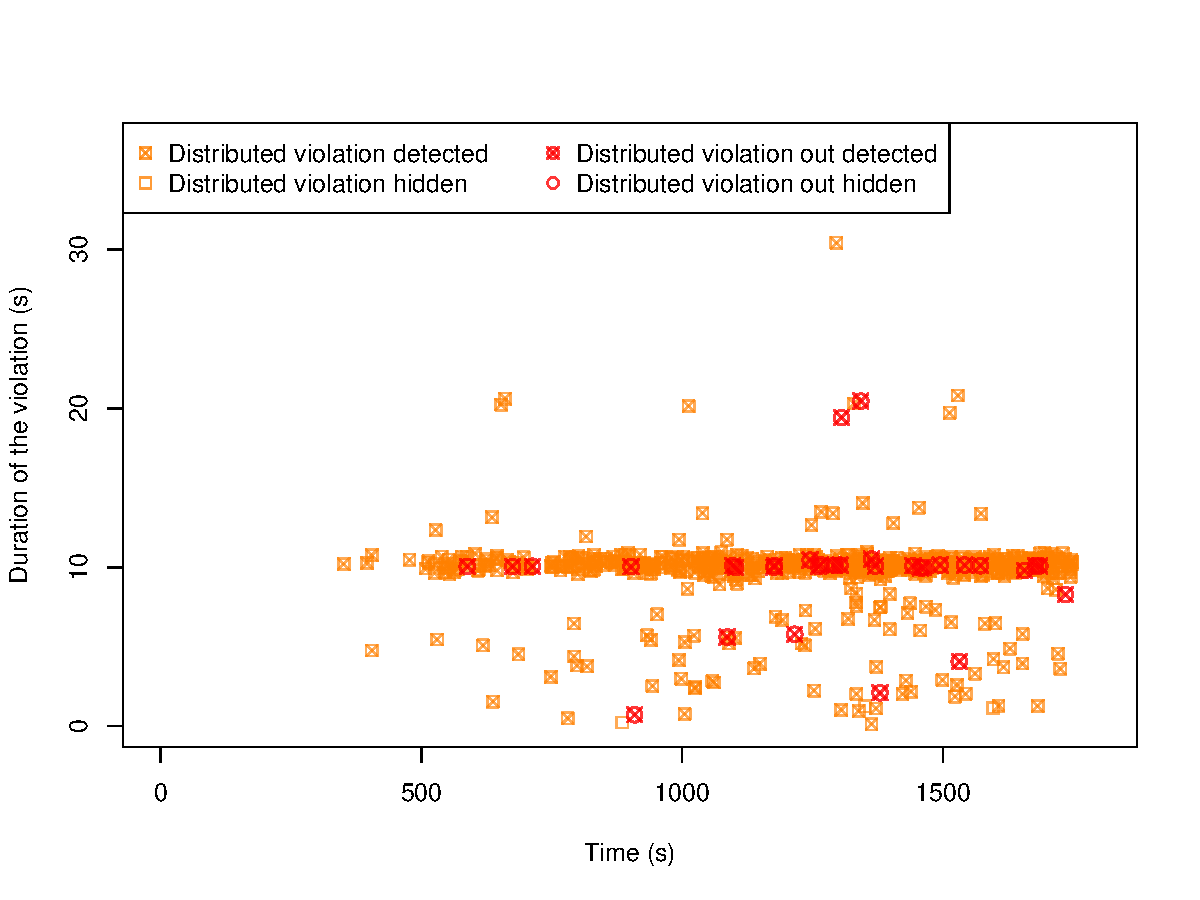
\includegraphics[width=.32\linewidth]{figures/experiments/clouds-1024-distributed.pdf}
  \label{fig:violation_clouds_dvms_1024}}
\subfigure[Snooze Periodic]{
  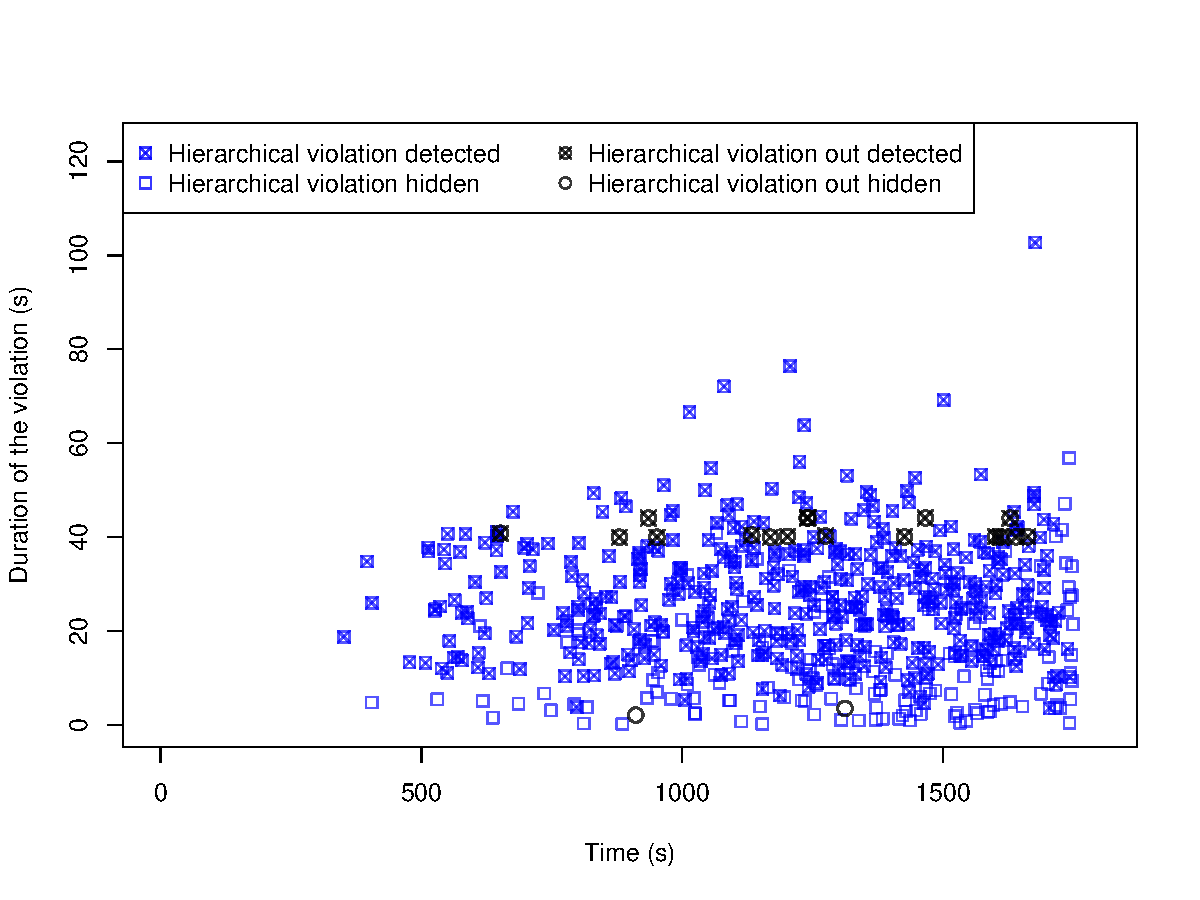
\includegraphics[width=.32\linewidth]{figures/experiments/clouds-1024-hierarchical-periodic-30-gm32.pdf}
  \label{fig:violation_clouds_snooze_1024_periodic}}
\subfigure[Snooze Reactive]{
  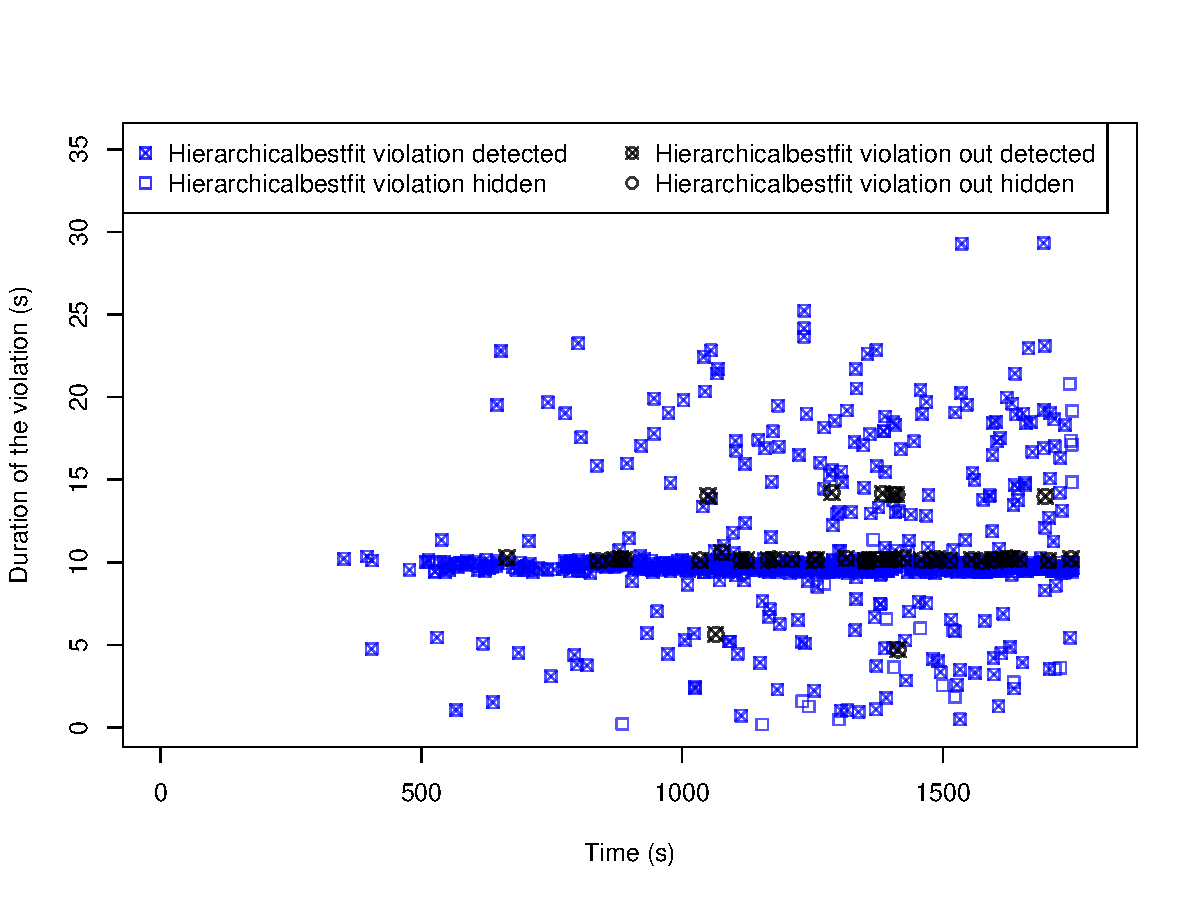
\includegraphics[width=.32\linewidth]{figures/experiments/clouds-1024-hierarchical-reactive-gm32.pdf}
  \label{fig:violation_clouds_snooze_1024_reactive}}
\caption{Details of violations duration occuring during simulation (10240 VMS).}
\label{fig:violation_clouds}
\end{figure*}
\AL[AL]{Figure \ref{fig:violation_clouds} should be discussed after
  the reactive discussion, the figure illustrates the pros of the reactivity.}
% \paragraph{Assignment of LCs to GMs}

% LCs are assigned to GMs by the GL as part of the LC join protocol. In
% Snooze's native implementation LCs are assigned in a round-robin
% fashion to the known GMs. If GMs join (and leave) the system at the
% same time as LCs, a round-robin (RR) strategy at join time, however,
% does not ensure an even distribution. This may happen, for instance at
% startup time of the system, when new GMs and LCs enter the system, or
% in case of failures, which trigger GM and LC joins. In order to
% evaluate the corresponding imbalance and its consequences we have
% implemented the LC assignment protocol in a modular fashion and
% applied it to different highly-dynamic settings in which GMs and LCs
% enter the system at the same time. Furthermore, we have implemented a
% best-fit (BF) strategy that assigns LCs to the GMs with minimal load
% or, if several GMs with minimal load exist, to the GMs with the
% smallest number of assigned LCs.


% % \subsubsection{LC assignment in Snooze-like placement alg.}
% % \label{sec:snoozeVariantsEval}

% % \begin{figure}[ht]
% % \begin{center}
% %     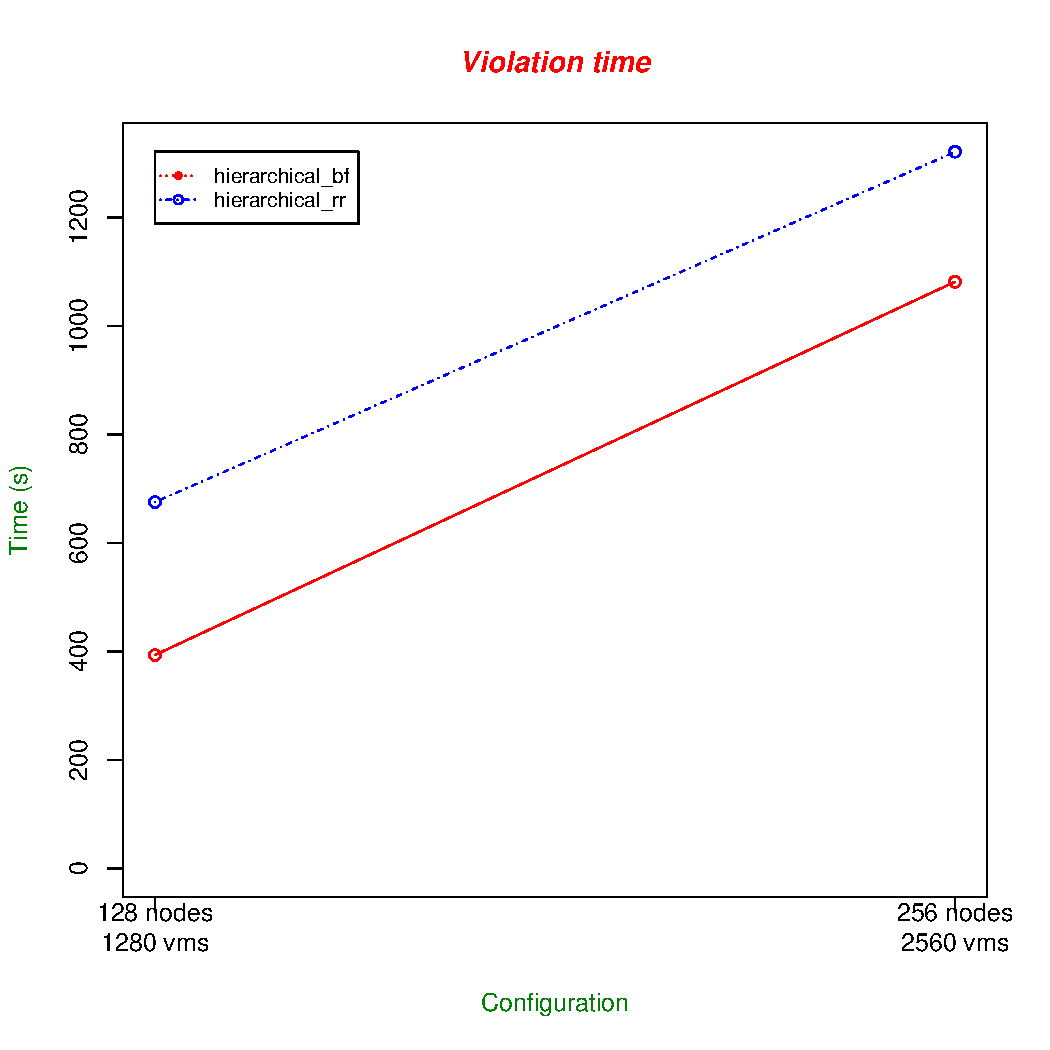
\includegraphics[width=.95\linewidth]{figures/violationTime-snooze-RR-BF.pdf}
% %     \caption{Cumulated violation time for BF (lower line) and RR
% %       (upper line) variants}
% % \end{center}
% % \label{fig:snoozeBFRRViolation}
% \end{figure}

% \begin{table*}[ht]
% \begin{center}
% %    \begin{tabular}{|c!{\vrule width 3pt}c|c|c!{\vrule width 2pt}c|c|c!{\vrule width 3pt}c|c!{\vrule width 2pt}c|c|}
%     \begin{tabular}{|P{30mm}|||c|c||c|c|||M{30mm}|M{30mm}|}
%         \thickhline
%         \multirow{3}*{\textbf{Strategy}}
%           & \multicolumn{4}{c|||}{\textbf{\#LCs/\#GMs}}
%           & \multicolumn{2}{c|}{\textbf{Total violation time (s)}}
%           \Tstrut \\
%           & \multicolumn{2}{c||}{128 LCs, 12 GMs}
%             & \multicolumn{2}{c|||}{256 LCs, 25 GMs}
%           & \multirow{2}*{128 LCs, 12 GMs} & \multirow{2}*{256 LCs, 25 GMs}
%           \Bstrut \\
%           & range & stdev & range & stdev & &  \Bstrut \\
%         \thickhline
%         Best-Fit & 0--30 & 10.53 & 0--18 & 6.62  & 395 & 1005 \Rstrut \\
%         Round-Robin & 0--49 & 15.7  & 0--35 & 12.22 & 630 & 1265
%         \Rstrut \\ \hline
%         \thickhline
%     \end{tabular}
% \end{center}
%     \caption{LCs to GM assignment and cumulated violation times for RR
%       and BF strategies}
%     \label{tbl:assignmentResults}
% \end{table*}


% We have evaluated the two LC assignment strategies using \vmps on
% configurations of~128 and~256 nodes. In order to clearly expose the
% corresponding differences this evaluation has been performed by
% ``stressing'' the two strategies by simultaneously
% starting all LCs (128/256) and all GMs (12/25) and then simulating the
% resulting configuration over a one hour period.  These experiments
% have yielded the following results, cf.\ Table~\ref{tbl:assignmentResults}:
% \begin{itemize}
%   \item BF yields more homogeneous assignments of LCs to GMs: the
%     ranges of the numbers of LCs assigned to a GM and their standard
%     deviations are significantly smaller.\footnote{Here, some GMs may
%       be assigned 0 LCs if some GMs join the system after all LCs have
%       been assigned.}
%   \item The cumulated time spent resolving violations is, for both
%     configurations, significantly smaller for BF than for RR.
% \end{itemize}
% From these results, we can clearly infer that BF is significantly
% better than RR for the two tested kinds of configuration. Furthermore,
% we conjecture that BF should perform at least as good as RR for all
% configurations (the proof is left to future work).
% % \MS[JP]{I need the exact figures for the violation times
% %   in Tbl.~\ref{tbl:assignmenResults}}

% \paragraph{Variants of the join algorithms}

% The join algorithms, see Sec.~\ref{sec:snoozeAlgs}, are crucial to
% Snooze for two main reasons: (i) they have to be efficient because
% they can easily form a bottleneck if large numbers of LCs (GMs) have
% to be registered at a GM (LC); (ii) they are multi-phase protocols
% whose correctness especially in the presence of faults is difficult to
% ensure.

% In order to investigate the corresponding trade-offs, we have used our
% framework to implement join algorithms that may be interrupted at any
% time, repeat the the on-going phase a number of times before
% reinitiating, if necessary, the entire protocol. Furthermore, the join
% protocol is parameterized, \eg, in the number of threads used to
% handle registration requests.

% Finally, our framework has enabled us to test another aspect of
% Snooze's join algorithm as presented by
% Feller~\etal.~\cite{feller:ccgrid12}, a strategy we call the GM rejoin
% strategy (GRJ): all GMs and the LCs assigned to them should rejoin if
% a new GM enters the system. While GRJ supports a form of load
% balancing (because all LCs are reassigned to the new set of GMs), our
% simulation has shown that this strategy significantly increases the
% time necessary for registering GMs and LCs compared to a simpler
% strategy that does not modify existing GMs in case a new GM enters the
% system. This handicap is particularly pronounced if joins of GMs may
% be interrupted due to faults. Concretely, experiments involving 20 GMs
% and 200 LCs have shown that this strategy often multiplies the time
% necessary to join all 220 components by 10 or more compared to the
% simple join strategy. While the qualitative result that the more
% complex strategy presented in the paper results in a more
% time-consuming join process is not very surprising, the extent of the
% resulting degradation was surprising.



\subsubsection{DVMS Analysis}
\AL{For the journal: add PajeGN view for DVMS}

In section \ref{sec:ISP}, the functioning of the iterative scheduling procedure
has been described: DVMS includes each overloaded node in a new partition, these
partitions will include new nodes, until a satisfactory reconfiguration implying
its members has been found. As, in the original design of DVMS, partitions had
no size constraint, it was interesting for us to verify if adding such a
constraint would have an impact on its behaviour.

% \begin{figure}
% \subcapcentertrue
% \subfigure[Migration count]{
%   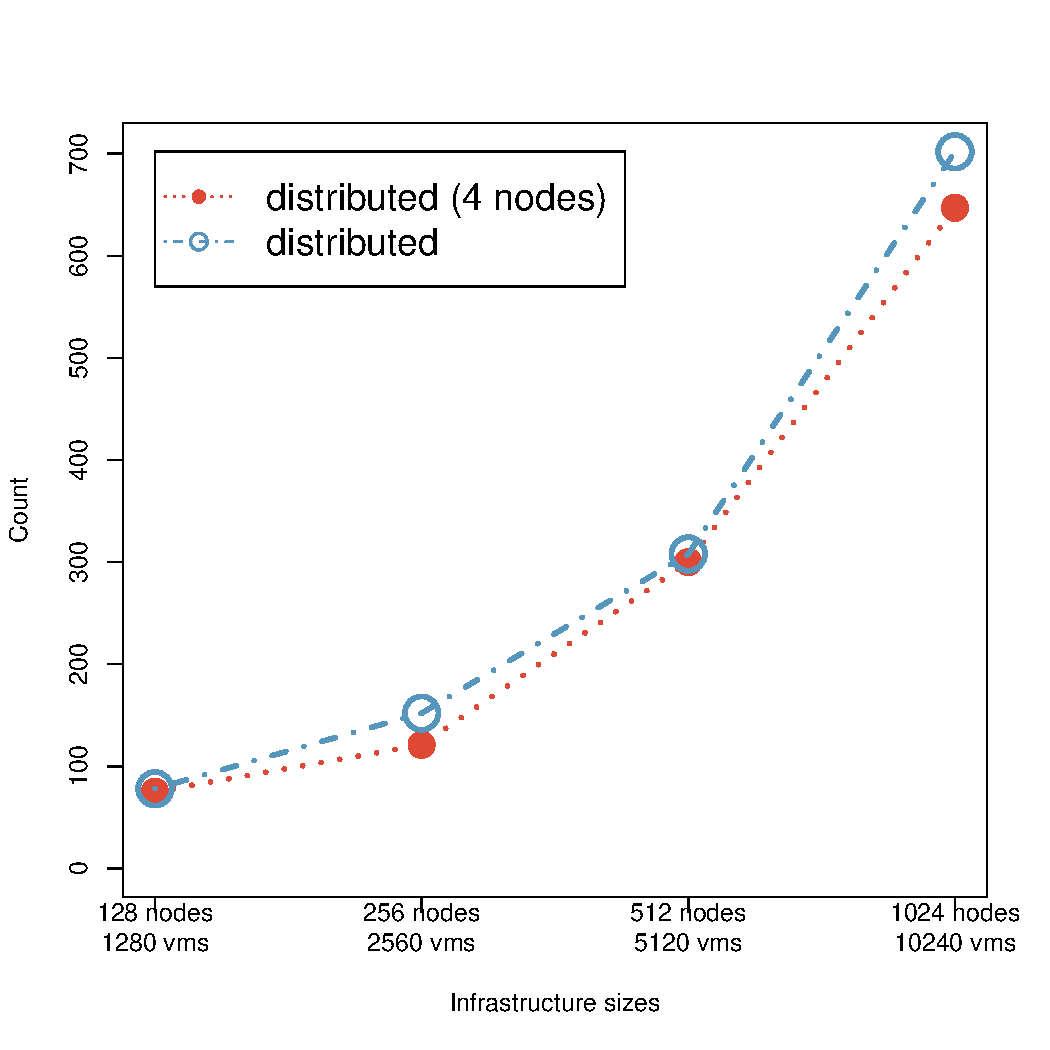
\includegraphics[width=.47\linewidth]{figures/experiments/dvms_comparison_migration_count.pdf}
%   \label{fig:dvms_comparison_migration_count}}
% \subfigure[Cumulated violation duration]{
%   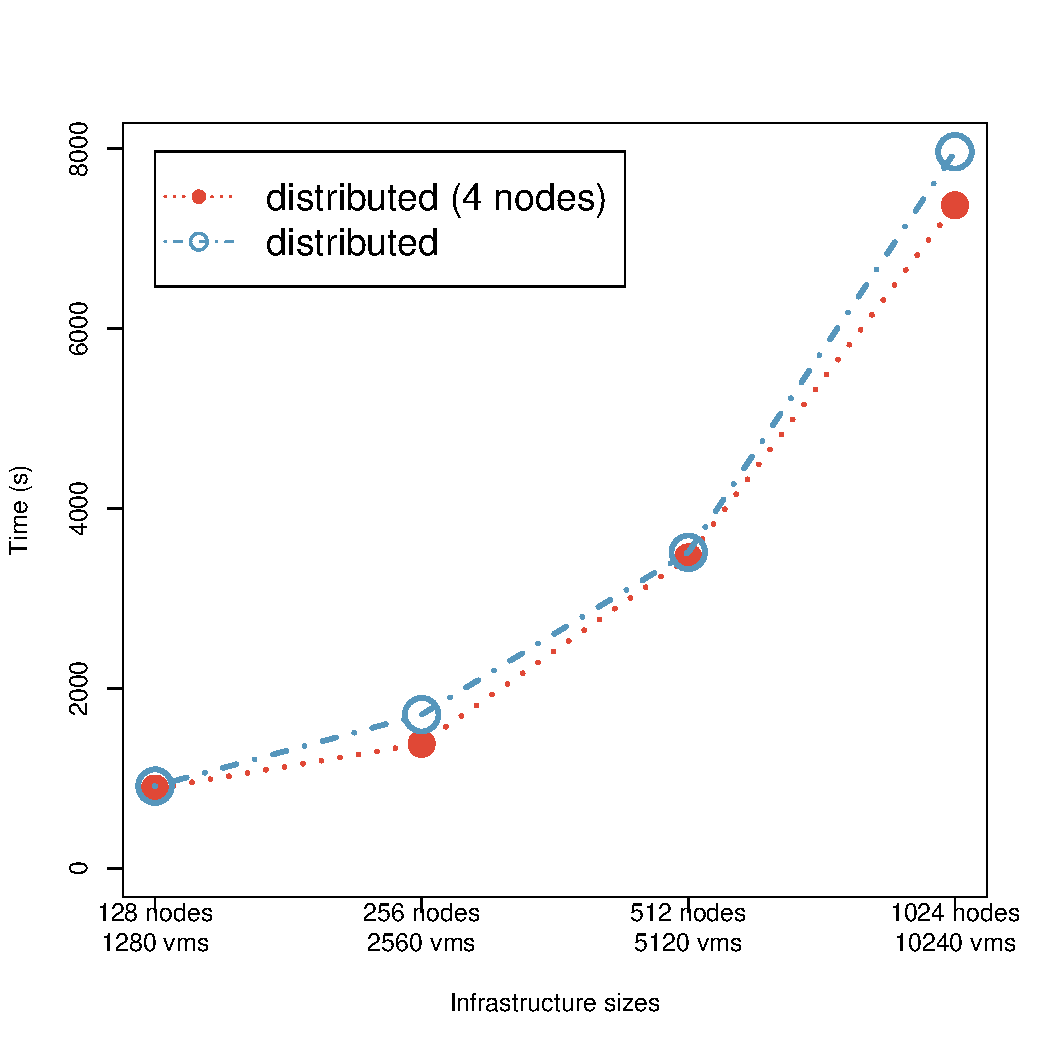
\includegraphics[width=.47\linewidth]{figures/experiments/dvms_comparison_violation_duration.pdf}
%   \label{fig:dvms_comparison_violation_duration}}
% \caption{Comparison of two flavours of DVMS}
% \label{fig:violation_clouds}
% \end{figure}

\begin{table}[ht]
\centering
    {\scriptsize \begin{tabular}{|P{27mm}@{\:}||@{\:}c@{\:}|@{\:}c@{\:}||@{\:}c@{\:}|@{\:}c@{\:}|}
      \thickhline
      \textbf{Infrastructure Size}
        & \multicolumn{2}{c@{\:}||@{\:}}{\textbf{No.\ migrations}}
        & \multicolumn{2}{c@{\:}|}{\textbf{Violation time (s)}}
          \Tstrut \\
         \hfill flavour &  ~Original~ & 4 nodes  &  ~Original~ & 4 nodes \Bstrut \\
      \thickhline

        128 nodes &   78  & 76  & 914.28  & 884.46  \\
        256 nodes &   152 & 127 & 1709.23 & 1498.71 \\
        512 nodes &   308 & 286 & 3513.18 & 3314.72 \\
       1024 nodes &   702 & 616 & 7967.03 & \:7101.49

      \Rstrut  \\ \hline
      \thickhline
  \end{tabular} }
\caption{Comparison of two DVMS flavours.}
\label{tab:dvms_flavours}
\end{table}

% {\scriptsize \begin{tabular}{|P{27mm}@{\:}||@{\:}c@{\:}|@{\:}c@{\:}|@{\:}c@{\:}||@{\:}c@{\:}|@{\:}c@{\:}|@{\:}c@{\:}|}
%     \thickhline
%     \textbf{Algorithm}
%       & \multicolumn{3}{c@{\:}||@{\:}}{\textbf{No.\ migrations}}
%       & \multicolumn{3}{c@{\:}|}{\textbf{Violation time (s)}}
%         \Tstrut \\
%        \hfill\#LCs  & ~128~ & ~256~ & 512 & ~~128~~ & ~~256~~ & 512 \Bstrut \\
%     \thickhline
%       Reactive      & 107 & 201 & 421 & 1075 & 1955 & 4385 \\
%       Periodic 30s  & 62 & 124 & 269 & 1770 & 3453 & \:8196
%     \Rstrut  \\ \hline
%     \thickhline
% \end{tabular}

% \caption{Influence of the Snooze group size ($Med\pm \sigma$)}
% \label{tab:dvms_flavours}
% }


% \begin{figure}[ht]
% \begin{center}
%     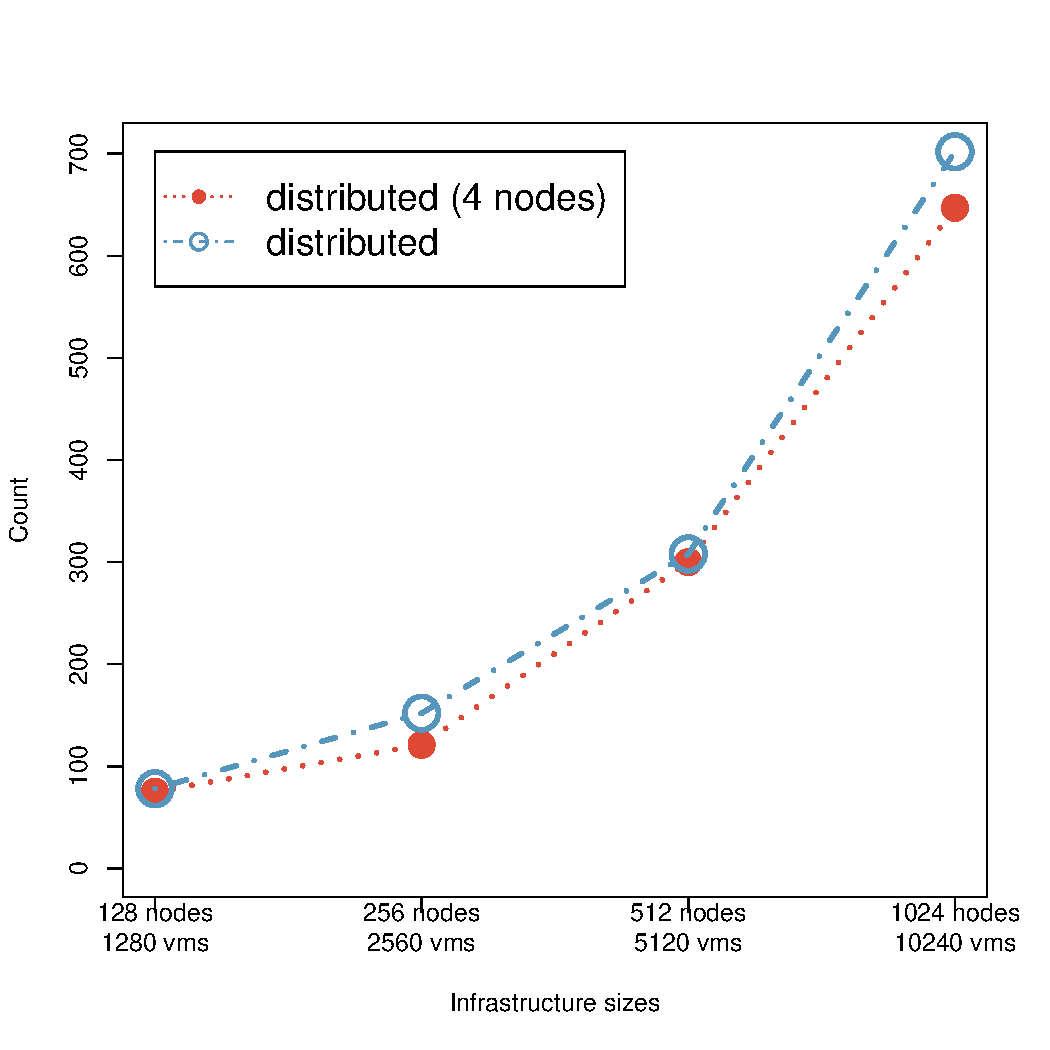
\includegraphics[width=.65\linewidth]{figures/experiments/dvms_comparison_migration_count.pdf}
%     \caption{Comparison of two flavour of DVMS (migration count).}
%     \label{fig:dvms_comparison_migration_count}
% \end{center}
% \end{figure}

In Table \ref{tab:dvms_flavours}, we compared two implementations of
DVMS: one that complies the description given in Section \ref{sec:ISP} and one
that works on partitions which contain at least 4 nodes. It is noticeable that
the number of migrations is slightly smaller with the implementation that works
with at least 4 nodes. This is due to the quality of reconfiguration plans: as
more nodes can be used to rebalance the VMs workload, its quality can be
improved.

% \begin{figure}[ht]
% \begin{center}
%     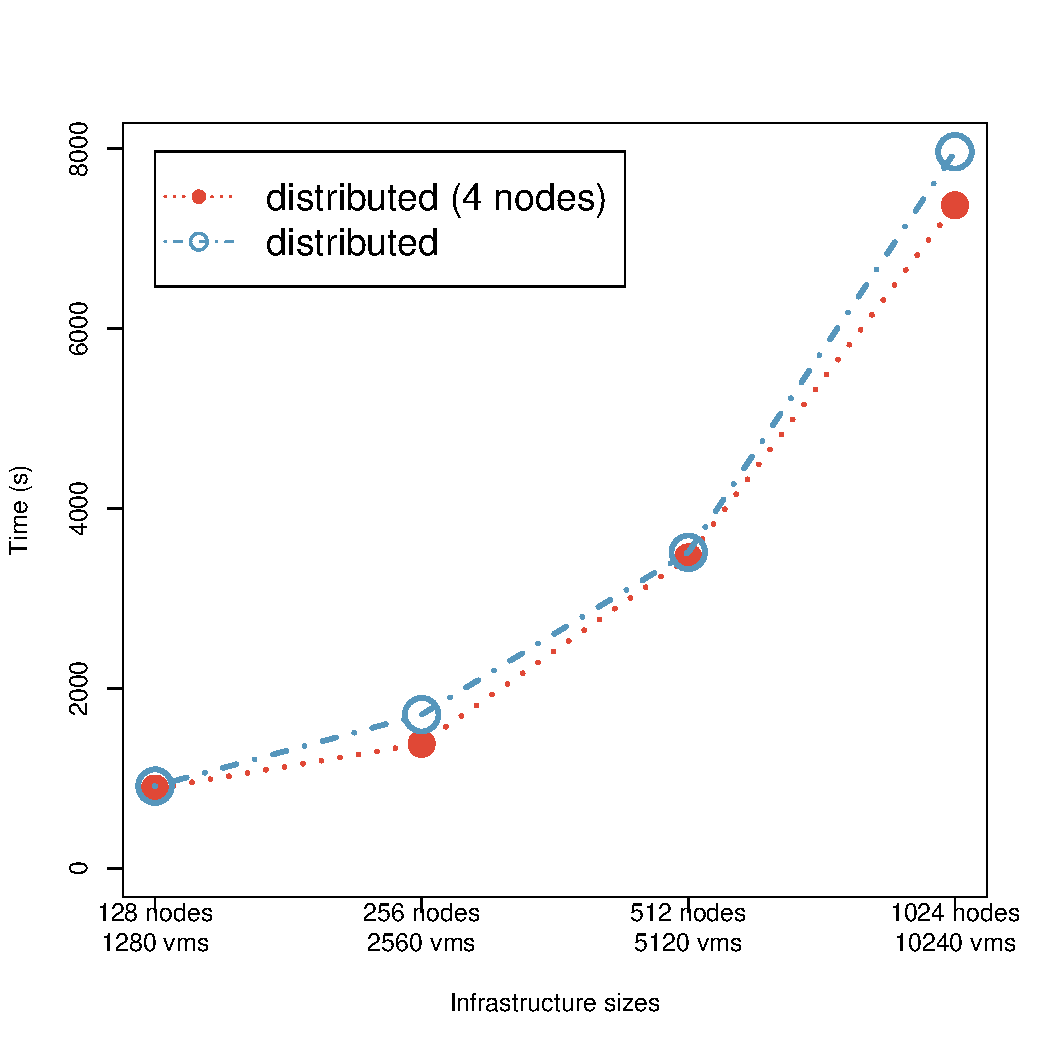
\includegraphics[width=.65\linewidth]{figures/experiments/dvms_comparison_violation_duration.pdf}
%     \caption{Comparison of two flavour of DVMS (cumulated violation time).}
%     \label{fig:dvms_comparison_violation_duration}
% \end{center}
% \end{figure}

Table \ref{tab:dvms_flavours} also shows that the preceding
fact has a direct impact on the VMs QoS: the cumulated violation duration
is reduced in the same proportion as the reduction of migrations.
% The comparison of different flavours of the DVMS algorithm is eased by the use
% of the VMPlaceS framework.




\section{Related Work}
\label{sec:related}
%\AL[AL]{Add few lines related to Google scheduling simulator - https://code.google.com/p/cluster-scheduler-simulator/}
%\AL[AL]{Add few lines about FlexCloud - http://arxiv.org/pdf/1501.05789v1.pdf}
Several simulator toolkits have been proposed since the last years in
order to adress CC concerns~\cite{CC13,DGSIM,cloudsim,icancloud,greencloud}.  They can be classified into two categories: The first
one corresponds to ad-hoc simulators that have been developped to
address a particular concern. For instance, CReST~\cite{CC13} is a
discrete event simulation toolkit built to evaluate Cloud provisioning
algorithms. If ad-hoc simulators enable to provide some trends
regarding the bevahiours of the system, they do consider the
implication of the different layers, which can lead to non
representative results at the end. Moreover, such ad-hoc solutions are
developped for one shot and thus, they are not available for the
scientific community. The second category \cite{icancloud,greencloud,
  cloudsim} corresponds to more generic cloud simulator toolkits (\ie
they have been designed to adress a majority of CC
challenges). However, they have focused mainly on the API and not on
the model of the different mechanisms of CC systems.

For instance, CloudSim~\cite{cloudsim}, which has been widely used to
validate algorithms and applications in different scientific
publications, is based on a relatively top-down viewpoint of cloud
environments.  That is, there is no papers that properly validate the
different models it relies on: a migration time is calculated by
dividing a VM memory size by a network bandwidth.
%Such a model cannot correctly simulate many real
%environments where workloads perform substantial memory writes.
 In addition to having inaccuracy weaknesses at the low level, available cloud
simulator toolkits over simplified the model for the virtualization
technologies, leading also to non representation results at the
end. As highlighted several times throughout this document, we chose to
build \vmps on top of \sg in order to benefit fromt its accuracy of
its models related to virtualization abstractions~\cite{Hirofuchi:2013:ALM:2568486.2568524}.


Cloud Computing has entered our everyday life at a very high speed and huge scale. From classic high performance computing simulations to the management of huge amounts of data coming from mobile devices and sensors, its impact can no longer be minimized. While a lot of progress has already been made in Cloud technologies, there are several concerns that limit the complete adoption of the Cloud Computing paradigm.

In a previous report~\cite{lebre:hal-00854204}, we outlined that, in addition to these concerns, the current model of UC is limited by intrinsic issues. Instead of following the current trend by trying to cope with existing platforms and network interfaces, we proposed to take a different direction by promoting the design of a system that will be efficient and sustainable at the same time, putting knowledge and intelligence directly into the network backbone itself. The innovative approach we introduced will definitely tackle and go beyond Cloud Computing limitations. Our objective is to pave the way for a new generation of Utility Computing that better matches the Internet structure by means of advanced operating mechanisms. By offering the possibility to tightly couple UC servers and network backbones throughout distinct sites and operate them remotely, the LUC OS technology may lead to major changes in the design of UC infrastructures as well as in their environmental impact. The internal mechanisms of the LUC OS should be topology dependent and resources efficient. The natural distribution of the nodes through the different points of presence should be an advantage, which allows to process a request according to its scale: Local requests should be computed locally, while large computations should benefit from a large number of nodes.

The first step toward this highly distributed Cloud infrastructure taking into account locality and network distance is the scheduling of VMs taking into account locality. Thus is this paper, we presented our first building block of our distributed Cloud infrastructure that consists in using P2P algorithms and a vivaldi overlay connected to DVMS, an efficient and flexible VMs scheduler. Our first experiments over Grid'5000 show that, connecting 4 differents sites and scheduling VMs over them, we can gain up to 66\% of inter-sites operations. 

Our future work will consist in ... 


%\bibliographystyle{abbrv}
%\bibliography{refs}

%\appendices
%%%%%%%%%%%%%%%%%%%%%% appendix.tex %%%%%%%%%%%%%%%%%%%%%%%%%%%%%%%%%
%
% sample appendix
%
% Use this file as a template for your own input.
%
%%%%%%%%%%%%%%%%%%%%%%%% Springer-Verlag %%%%%%%%%%%%%%%%%%%%%%%%%%

\chapter{Chapter Heading}
\label{introA} % Always give a unique label
% use \chaptermark{}
% to alter or adjust the chapter heading in the running head

Use the template \emph{appendix.tex} together with the Springer document class SVMono (monograph-type books) or SVMult (edited books) to style appendix of your book in the Springer layout.


\section{Section Heading}
\label{sec:A1}
% Always give a unique label
% and use \ref{<label>} for cross-references
% and \cite{<label>} for bibliographic references
% use \sectionmark{}
% to alter or adjust the section heading in the running head
Instead of simply listing headings of different levels we recommend to let every heading be followed by at least a short passage of text. Further on please use the \LaTeX\ automatism for all your cross-references and citations.


\subsection{Subsection Heading}
\label{sec:A2}
Instead of simply listing headings of different levels we recommend to let every heading be followed by at least a short passage of text. Further on please use the \LaTeX\ automatism for all your cross-references and citations as has already been described in Sect.~\ref{sec:A1}.

For multiline equations we recommend to use the \verb|eqnarray| environment.
\begin{eqnarray}
\vec{a}\times\vec{b}=\vec{c} \nonumber\\
\vec{a}\times\vec{b}=\vec{c}
\label{eq:A01}
\end{eqnarray}

\subsubsection{Subsubsection Heading}
Instead of simply listing headings of different levels we recommend to let every heading be followed by at least a short passage of text. Further on please use the \LaTeX\ automatism for all your cross-references and citations as has already been described in Sect.~\ref{sec:A2}.

Please note that the first line of text that follows a heading is not indented, whereas the first lines of all subsequent paragraphs are.

% For figures use
%
\begin{figure}[t]
\sidecaption[t]
% Use the relevant command for your figure-insertion program
% to insert the figure file.
% For example, with the graphicx style use
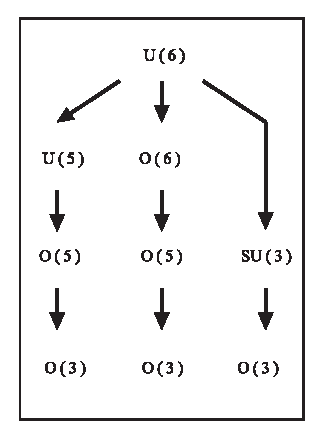
\includegraphics[scale=.65]{figure}
%
% If no graphics program available, insert a blank space i.e. use
%\picplace{5cm}{2cm} % Give the correct figure height and width in cm
%
\caption{Please write your figure caption here}
\label{fig:A1}       % Give a unique label
\end{figure}

% For tables use
%
\begin{table}
\caption{Please write your table caption here}
\label{tab:A1}       % Give a unique label
%
% Follow this input for your own table layout
%
\begin{tabular}{p{2cm}p{2.4cm}p{2cm}p{4.9cm}}
\hline\noalign{\smallskip}
Classes & Subclass & Length & Action Mechanism  \\
\noalign{\smallskip}\hline\noalign{\smallskip}
Translation & mRNA$^a$  & 22 (19--25) & Translation repression, mRNA cleavage\\
Translation & mRNA cleavage & 21 & mRNA cleavage\\
Translation & mRNA  & 21--22 & mRNA cleavage\\
Translation & mRNA  & 24--26 & Histone and DNA Modification\\
\noalign{\smallskip}\hline\noalign{\smallskip}
\end{tabular}
$^a$ Table foot note (with superscript)
\end{table}
%


\subsubsection{Acknowledgments.}
Experiments presented in this paper were carried out using the Grid'5000 experimental
testbed, being developed under the INRIA ALADDIN development action with support from
CNRS, RENATER, and several Universities as well as other funding bodies (see
\url{https://www.grid5000.fr}).

\bibliographystyle{llncs2e/splncs03}
\bibliography{main}

\end{document}
